\documentclass[a4paper,11pt,oneside,openany,report]{jsbook}

\usepackage[left=30mm,right=30mm,top=25mm,bottom=25mm]{geometry}
\usepackage{cscover}
\usepackage[nobreak]{cite}
\usepackage[a4paper,dvipdfmx,pdfdisplaydoctitle=true,%
    bookmarks=true,bookmarksnumbered=true,bookmarkstype=toc,bookmarksopen=true,%
    pdftitle={スケーラブルかつ高精度なSpectre脆弱性の検出手法},%
    pdfauthor={吉田昂太}%
    ]{hyperref}
\usepackage{pxjahyper}
\usepackage{indentfirst}
%%%%%%%%%%%%%%%%%%%%%%%%%%%%%%%%%%%%%%%%%%%%%%%%%%
%% global package settings, macros
%%%%%%%%%%%%%%%%%%%%%%%%%%%%%%%%%%%%%%%%%%%%%%%%%%

\usepackage[dvipdfmx]{graphicx}
\usepackage{latexsym}
\usepackage{listings}
\usepackage{minted}
\usepackage{mdframed}
\usepackage{caption}
\usepackage{algpseudocode}
\usepackage{algorithm}
\usepackage{color}
\usepackage{ulem}
\usepackage{url}
\usepackage{subcaption}
\usepackage {amsmath}
\usepackage{stmaryrd}
\usepackage{amsthm}
\usepackage{amsmath, amssymb}
\usepackage{booktabs}
\usepackage{multirow}
\usepackage {threeparttable}
\usepackage{spreadtab}
\usepackage{xcolor}

% \definecolor{mygreen}{rgb}{0,0.6,0}
% \definecolor{mygray}{rgb}{0.5,0.5,0.5}
% \definecolor{mymauve}{rgb}{0.58,0,0.82}

\definecolor{highlightDel}{RGB}{249,216,214}
\definecolor{highlightAdd}{RGB}{177,239,196}

% ハイライト用のコマンドを定義
\newcommand{\del}[1]{\colorbox{highlightDel}{#1}}
\newcommand{\add}[1]{\colorbox{highlightAdd}{#1}}

% settings for minted
\newenvironment{code}{\captionsetup{type=listing}}{}
\mdfdefinestyle{mystyle}{
  linecolor=black,
  topline=true,
  bottomline=true,
  leftline=true,
  rightline=true,
  innertopmargin=2pt,
  innerbottommargin=3pt,
  innerleftmargin=3pt,
  innerrightmargin=2pt,
  roundcorner=4pt
}
\surroundwithmdframed[style=mystyle]{minted}

% settings for listing
\lstset{
  basicstyle={\ttfamily},
  breaklines=true,
  captionpos=b,
  columns=[l]{fullflexible},
  commentstyle={\smallitshape},
  frame={single},
  identifierstyle={\small},
  keywordstyle={\small\bfseries},
  lineskip=-0.5ex,
  ndkeywordstyle={\small},
  numbers=left,
  numbersep=1zw,
  numbersep=5pt,
  numberstyle={\scriptsize},
  stepnumber=1,
  stringstyle={\small\ttfamily},
  xleftmargin=3zw,
  xrightmargin=0zw,
}

\newtheorem{definition}{定義}

% macros for algorithm
\algnewcommand{\algorithmicand}{\textbf{ and }}
\algnewcommand{\algorithmicor}{\textbf{ or }}
\algnewcommand{\algorithmicnot}{\textbf{ not }}
\algnewcommand{\OR}{\algorithmicor}
\algnewcommand{\AND}{\algorithmicand}
\algnewcommand{\NOT}{\algorithmicnot}
\algnewcommand{\var}{\texttt}

% macros for color
\newcommand*{\todo}[1]{\textcolor{magenta}{\textbf{todo:#1}}}
\newcommand*{\memo}[1]{\textcolor{magenta}{memo: #1}}


\renewcommand{\bibname}{参考文献}
\setcounter{tocdepth}{2}
\pagestyle{plain}

\newcommand{\TODO}[1]{\textbf{[TODO: #1]}}
%\renewcommand{\TODO}[1]{}

\thesistype{修士論文}
\title{スケーラブルかつ高精度な\\Spectre脆弱性の検出手法}
\author{吉田 昂太}
\studentid{23M30767}
\affiliation{東京科学大学\\情報理工学院\\情報工学系\\情報工学コース} 
\date{2025年1月}

\supervisorname{指導教員}
\supervisor{権藤 克彦}
%\dsupervisorname{副指導教員}
%\dsupervisor{工学 次郎}

% デフォルトの定義を保存
\let\oldsection\section
\let\oldsubsection\subsection
\let\oldsubsubsection\subsubsection
% \let\oldsection*\section*
% \let\oldsubsection*\subsection*
% \let\oldsubsubsection*\subsubsection*

% 定義を上書き
\renewcommand{\section}[1]{\chapter{#1}}
\renewcommand{\subsection}[1]{\oldsection{#1}}
\renewcommand{\subsubsection}[1]{\oldsubsection{#1}}
% \renewcommand{\section*}[1]{\chapter*{#1}}
% \renewcommand{\subsection*}[1]{\oldsection*{#1}}
% \renewcommand{\subsubsection*}[1]{\oldsubsection*{#1}}

\begin{document}

\frontmatter
\maketitle

%%%%%%%%%%%%%%%%%%%%%%%%%%%%%%%%%%%%%%%%%%%%%%%%%%
%% 概要
%%%%%%%%%%%%%%%%%%%%%%%%%%%%%%%%%%%%%%%%%%%%%%%%%%
\section{概要}
多くの CPU は投機的実行を悪用する Spectre 攻撃に対して脆弱である。これに対処するため、プロ
グラム内の Spectre 攻撃に脆弱なコード片(ガジェット)を特定し、部分的に投機的実行を抑制す
る方法が提案されている。既存の記号実行を用いたガジェットの検出手法は、通常の実行パスに加
え、投機的実行パスも探索する必要があるため、状態空間が増大し、大規模なプログラムに対しス
ケールしない問題がある。本論文では、ガジェットの検出可能性の低い投機的状態の探索を回避す
ることで、記号実行のスケーラビリティを向上させる手法を提案する。さらに、探索されなかった
投機的状態はファジングにより探索し、スケーラビリティと精度の両立を図る。




\tableofcontents
\listoffigures
\listoftables

%%%%%%%%%%%%%%%%%%%%%%%%%%%%%%%%%%%%%%%%%%%%%%%%%%

\mainmatter

%%%%%%%%%%%%%%%%%%%%%%%%%%%%%%%%%%%%%%%%%%%%%%%%%%
%% はじめに
%%%%%%%%%%%%%%%%%%%%%%%%%%%%%%%%%%%%%%%%%%%%%%%%%%
\section{はじめに}




%%%%%%%%%%%%%%%%%%%%%%%%%%%%%%%%%%%%%%%%%%%%%%%%%%
%% 背景知識
%%%%%%%%%%%%%%%%%%%%%%%%%%%%%%%%%%%%%%%%%%%%%%%%%%
\section{背景}
\subsection{投機実行}
\label{sec:spec_exec}

現代のCPUは1つの命令を、命令フェッチ、デコード、実行などの複数のステージに分割して実行するパイプライン方式を採用している。この方式により、前の命令が全ての処理を終えることを待たずに、次の命令の処理を開始できる。このように複数の命令を並行して処理することでCPUはスループットを向上させている。\par
しかし、次に実行すべき命令が前の命令の実行結果に依存している場合、CPU は次にどの命令を実行するべきか判断できなくなり、命令の処理を一時的に停止させる必要がある。このような状況は制御ハザードと呼ばれ、CPUのパフォーマンスに大きな影響を与える可能性がある。このようなハザードによる命令の実行の停止(Stall)を回避するため、現代のCP は分岐命令に遭遇した場合、過去の実行結果に基づいて分岐先を予測することで、後続の命令を投機的に実行する。分岐予測による投機実行がどのように行われるかを図\ref{fig:Speculative_Execution}に示す。図\ref{fig:Speculative_Execution}に示すように、分岐予測に成功した場合、CPUはstallを回避し、効率的に命令を処理できる。一方、予測が失敗した場合は、投機実行した命令の結果を破棄し、正しい分岐方向から命令の実行を再開する必要がある。分岐先の予測には分岐予測器が用いられ、分岐命令のアドレスごとに過去の分岐方向を記録し、その情報から分岐先の予測を行う。\par
投機的に実行された命令と実行結果はCPU内部のReorder Buffer (ROB)という機構で管理される。ROBは、実行された命令が依存する他の命令の完了を待ちつつ、命令の実行順序を維持する役割を持つ。そのため、投機的に実行できる命令数はROBの大きさに制限されており、一般的には200命令程度のマイクロオペレーション ($\mu$OP)に制限される。分岐先が確定し予測が正しかった場合は、投機的実行の結果をレジスタやメモリなどのハードウェア状態に反映させる。一方、分岐先が誤っていた場合はROB内の投機的実行の結果を全て破棄し、誤った予測が行われた時点のアーキテクチャ状態までロールバックされる。\par

\begin{figure}[tb]
  \centering
  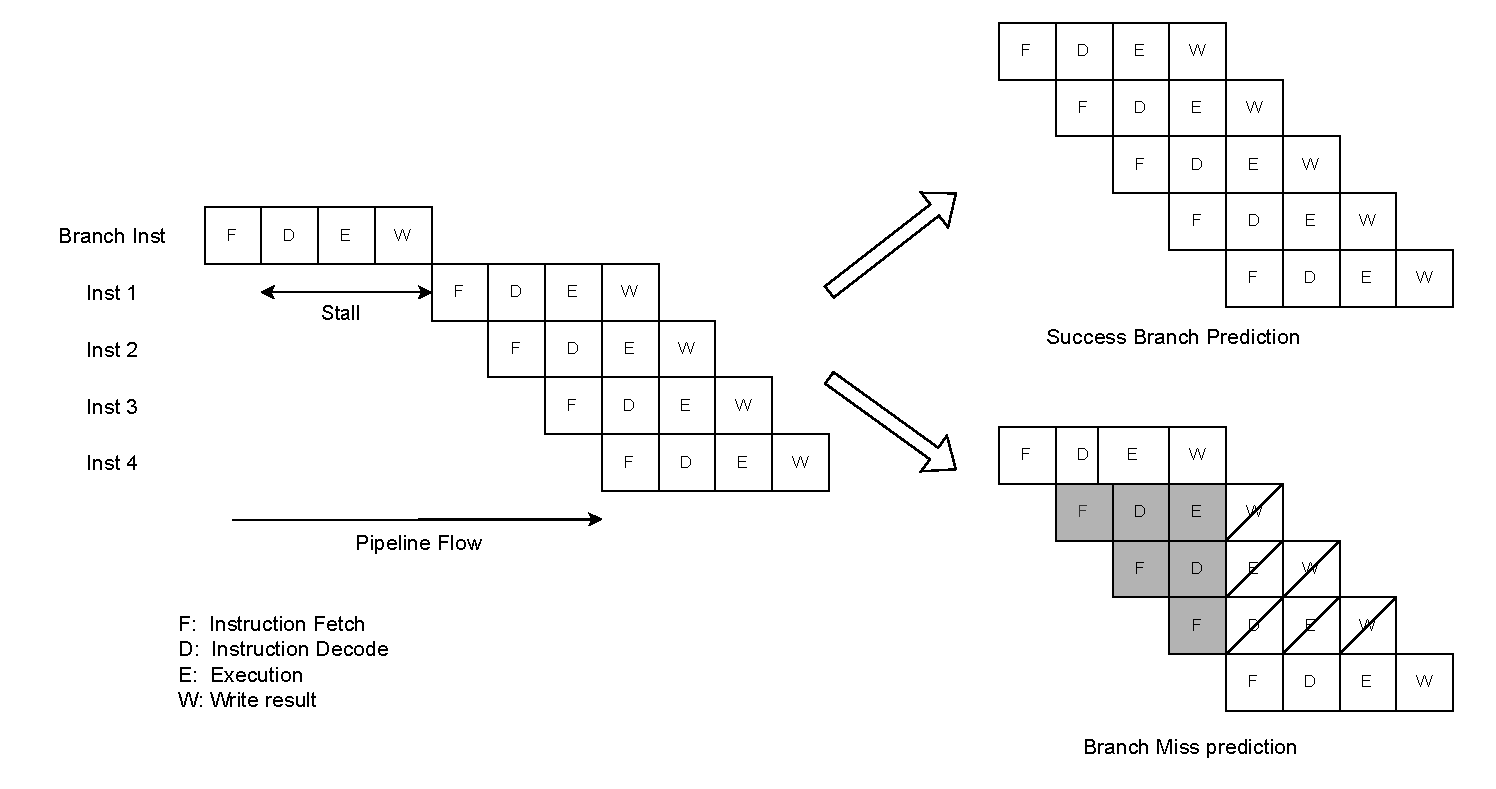
\includegraphics[width=\linewidth]{img/Speculative_Execution.drawio.pdf}
  \caption{分岐予測による投機実行}\label{fig:Speculative_Execution}
\end{figure}


\subsection{Side-Channel Attack}
コンピュータのシステムにおいて、channelとは情報を送信する可能性のある媒体のことを言う。channelには大きく分けてlegitimate channelと incidental channelの2種類が存在する\cite{intel-specter}。legitimate channelはシステムの設計者が情報送信用に意図したチャネルであり、イーサネット、共有メモリ、IPC ソケットなどがある。逆にincidental channelは 偶発的に設計されたチャネルであり、リソースの競合、CPU キャッシュの状態、電力消費の変化などがある。更に、セキュリティ脅威モデルのコンテキストにおいてincidental channelはcovert channelと side channelの2種類に分類される。covert channelは悪意のある送信者と受信者が意図的に情報の伝達を行うために利用されるchannelである。一方でside channelは、送信者は受信者に情報を伝達することを意図しておらず、情報が悪意のある受信者に伝達(つまり漏洩)される際に利用されるchannelであり、このようなchannelを悪用する攻撃手法をSide-Channel Attackという。\par 

side channel は 情報を伝達する方法に基づいて、Timing-based channel、Accessbased channel、またはTrace-based channel に分類できる\cite{szefer2019survey}。Timing-based channel は、様々な操作のタイミングを利用することで被害者の情報を推測する。例えば、攻撃者は様々な入力を暗号化または復号化し、その時の実行時間の差分を計測し分析することで、暗号鍵に関する情報が明らかになる可能性がある\cite{song2001timing}。Accessbased channels は メモリやキャッシュなどの共有リソースに直接アクセスすることで、被害者のプロセスの情報を推測する。例えば、キャッシュがプロセス間で共有されていることを利用し、特定のキャッシュラインへのアクセス時間を計測することで、被害者のプロセスの動作を推測することが出来る\cite{liu2015last}。Trace-based channels は デバイスの消費電力や電磁放射などのプログラム実行時の詳細な情報を計測することで情報の漏洩を試みる。例えば、攻撃者は暗号化中のデバイスの消費電力を計測し分析することで、暗号化に関する情報を収集する\cite{aciiccmez2006trace}。\par

以降の節では、近年のCPUのデータキャッシュの基本的な構造と、それを side channel として利用する代表的な攻撃手法である Prime+Probe\cite{tromer2010efficient} と Flush+Reload\cite{yarom2014flush+} について説明する。これらの攻撃は本研究の対象である、Spectre攻撃においても頻繁に利用される攻撃手法であるため、以降の節で詳しく説明する。

\subsubsection{キャッシュ構造}

\begin{figure}[tb]
  \centering
  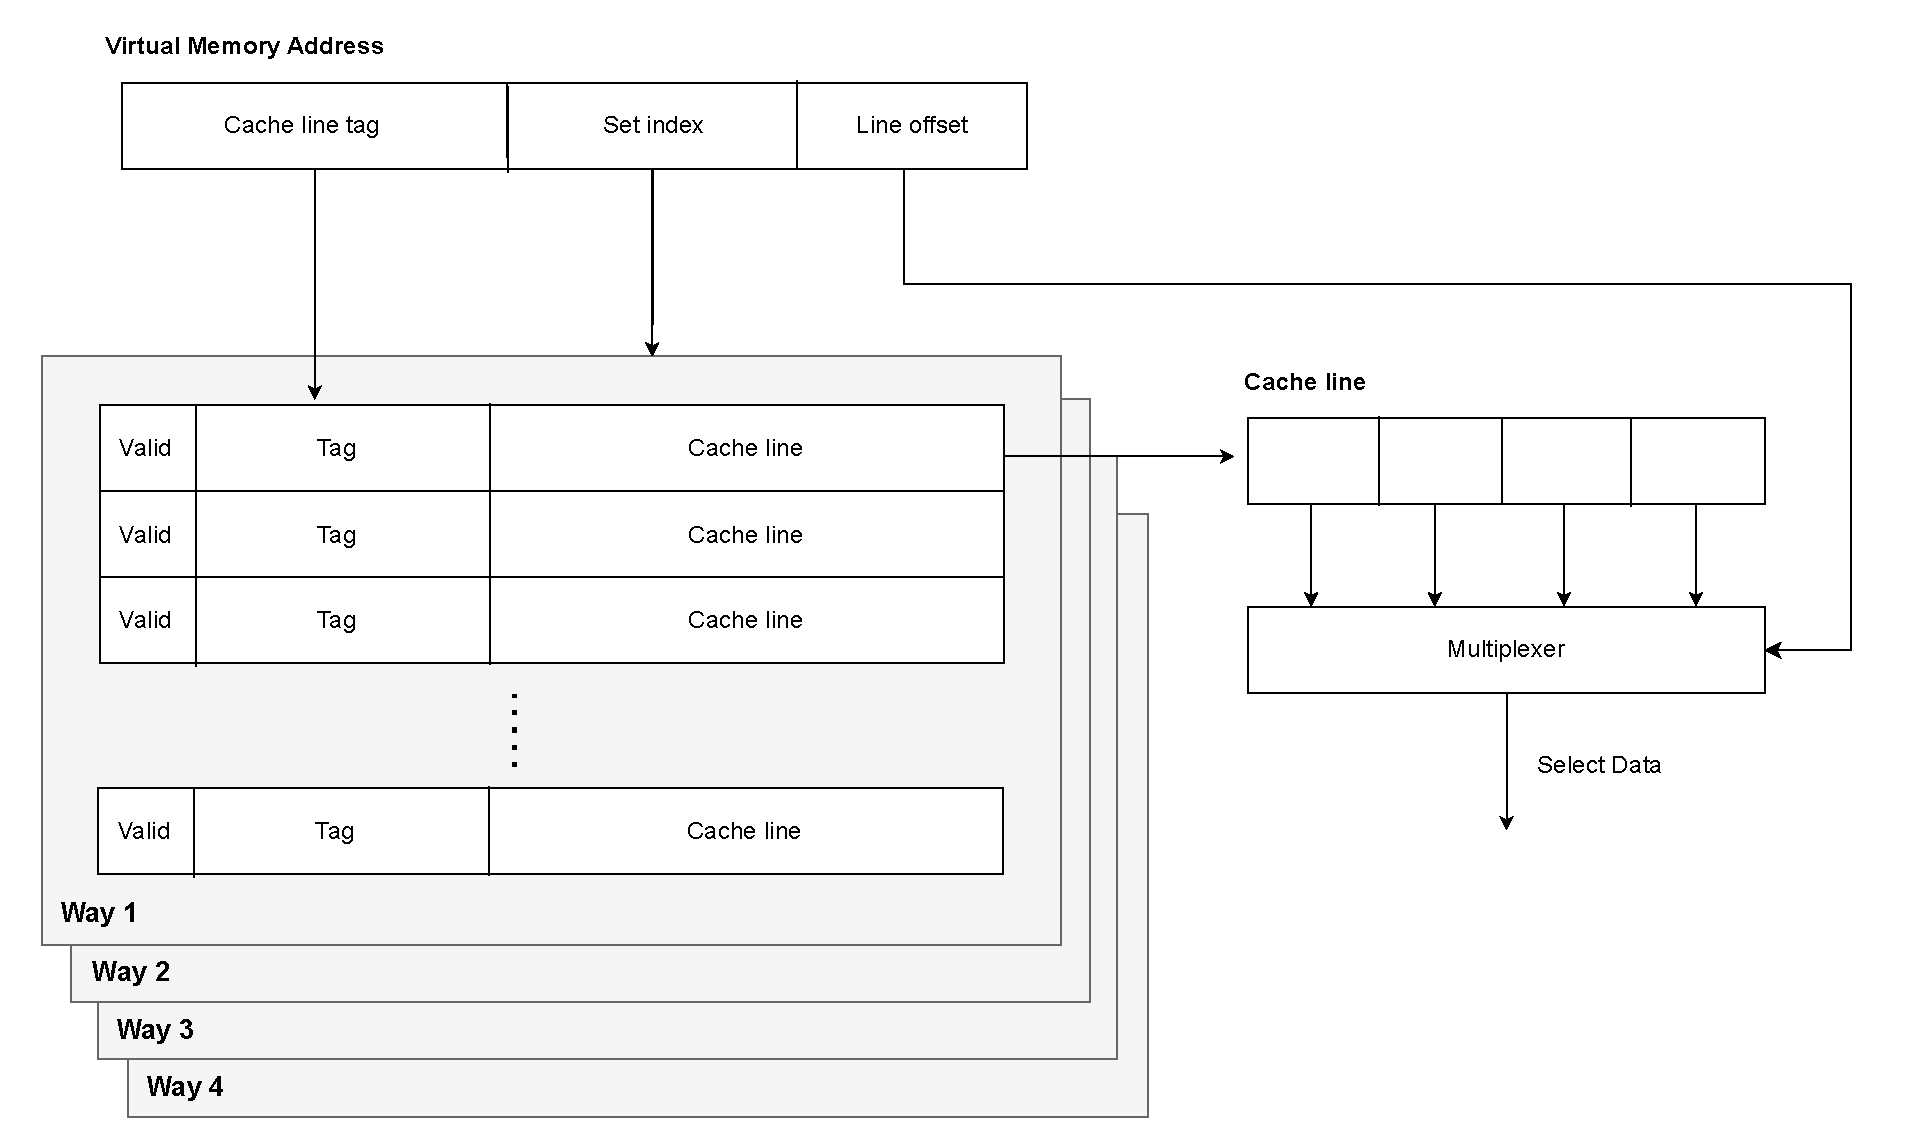
\includegraphics[width=\linewidth]{img/cache.drawio.pdf}
  \caption{仮想アドレスによるキャッシュの参照}\label{fig:cache-overview}
\end{figure}


キャッシュをside channelとして利用する攻撃手法を紹介する前に、近年のCPUにおけるキャッシュ構造について説明する。近年のCPUでは、プロセッサとメインメモリの性能差に効率的に対処するため、複数の性能が異なるキャッシュメモリを階層的に配置する設計が採用されている。このキャッシュ階層は、CPUに近い順にL1キャッシュ、L2キャッシュと続き、最も遠いキャッシュはLLC(Last Level Cache)と呼ばれる。これらのキャッシュはCPUに近いキャッシュほど高速だが容量が小さく、遠いほど容量は大きいが、低速であるという特徴を持つ。一般的にL1 キャッシュと L2 キャッシュは各コア専用で、LLCは複数のコアで共有されているため、LLCはSide-Channel Attackの対象として適している。\par

キャッシュは複数のキャッシュセットで構成され、各セットには複数のキャッシュラインが含まれている。このキャッシュ構造をセットアソシエイティブ型と呼び、各キャッシュセット内のキャッシュライン数を連想度(way)という。連想度が増加すると、キャッシュの競合性ミスが減少するが、比較器やキャッシュの設計コストが増加するため、バランスの取れた設計が求められる{\color{red}(TODO: intel CPUのway数は?)}。\par


仮想メモリアドレスは、以下の3つの要素で構成される。
\begin{itemize}
  \item Cache set index: キャッシュ内でデータがどのセットにマップされるかを決定する。
  \item Cache line tag: キャッシュセット内でデータを識別するタグ。
  \item Cache line tag: キャッシュライン内でどのデータワードが対象であるかを識別するタグ。
\end{itemize}

キャッシュは仮想アドレスの一部をインデックスとして使用し、各メモリアドレスを特定のキャッシュセットにマップする。そして、セット内の任意のキャッシュラインにデータを格納する。この際、マップ先のキャッシュセットがすでに埋まっている場合は、キャッシュ置換ポリシーに基づいて、どのキャッシュラインを削除するかが決定される。一般的に採用される手法は、Least Recently Used (LRU)やLeast Frequently Used (LFU)といったポリシーである。仮想メモリアドレスによる4wayセットアソシエイティブ型キャッシュの参照の概要を図\ref{fig:cache-overview}に示す。

\subsubsection{Prime+Probe}

\begin{figure}[tb]
  \centering
  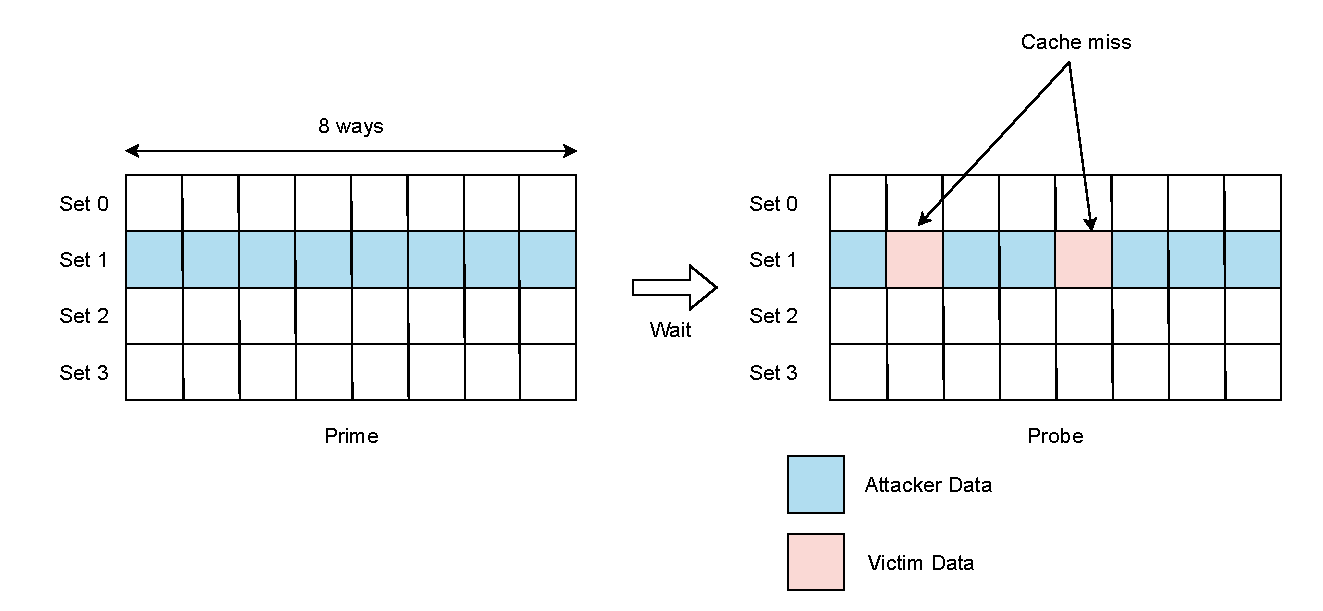
\includegraphics[width=\linewidth]{img/prime+probe.drawio.pdf}
  \caption{Prime+Probeの概要}\label{fig:prime-probe}
\end{figure}

Prime+Probe\cite{tromer2010efficient} は データキャッシュをside channelとして利用し、キャッシュ内の被害者のデータアクセスパターンから秘密情報を抽出する攻撃手法である。攻撃の概要について図\ref{fig:prime-probe}に示す。まず、攻撃者は、攻撃者プロセスにおけるコードブロックと被害者プロセスにおける機密性の高いコードブロックの両方がマップされるキャッシュセットを見つける。先述の通り、一部のキャッシュ階層は複数コア間で共有されているため、攻撃者と被害者のプロセスが同一コアにスケジュールされていなくても攻撃することは可能である\cite{liu2015last}。そして、攻撃者プロセスを一定時間実行することで、被害者と競合するキャッシュセットを自身のデータで埋める(Prime)。その後、攻撃者は一定時間待機し、被害者プロセスが実行されるのを待つ。これにより、競合したキャッシュセットの一部は被害者のデータによって上書きされる可能性がある。その後、攻撃者はPrimeフェーズで埋めたデータに再度アクセスし、アクセス時間を計測する(Probe)。アクセス時間を計測することで、攻撃者のデータがキャッシュ上に存在するかがわかるため、待機時間の間にどのキャッシュラインが被害者プロセスによってアクセスされたがわかる。つまり、攻撃者は特定のキャッシュセットにおける被害者プロセスのメモリアクセスパターンを把握することが可能となる。\par
Prime+Probeは後述するFlush+Reloadと比較して、フラッシュ命令や共有メモリを必要としないためより汎用的である。しかし、対象とするキャッシュがLLCのように大容量の場合、キャッシュセットを攻撃者のデータで埋めるまでに時間がかかるという欠点がある。

\subsubsection{Flush+Reload}
Flush+ReloadはPrime+Probeと同様に、データキャッシュを利用するSide-Channel攻撃であるが、前提条件として被害者と攻撃者のプロセス間で特定のメモリ領域を共有している必要がある。プロセス間でメモリを共有するシナリオとして、プロセス間通信のための利用される場合や、メモリフットプリントの削減のために、ハイパーバイザが仮想マシン間で同一内容のメモリページを結合する際に利用される\cite{yarom2014flush+}。\par
まず、攻撃者は共有されたメモリ領域の中から観測対象とするアドレスを選択し、clflush命令などを使用して、選択したアドレスのキャッシュラインをキャッシュ階層全体から排除する(Flush)。その後、攻撃者は一定時間待機し、被害者プロセスが観測対象のアドレスにアクセスするのを待つ。その後、攻撃者は観測対象のアドレスに再度アクセスし、アクセス時間を計測する(Reload)。待機中に被害者プロセスが観測対象のアドレスにアクセスした場合、そのキャッシュラインはキャッシュで利用可能になり、アクセス時間は短くなる。一方、被害者プロセスが観測対象のアドレスにアクセスしていない場合、キャッシュラインをメモリから取得する必要があるため、アクセス時間は長くなる。このようにして、攻撃者は待機中に被害者プロセスが観測対象のアドレスにアクセスしたかどうかを把握することが可能となる。\par
Flush+Reloadは攻撃のために前提条件が必要だが、Prime+Probeと比較して特定のアドレスのキャッシュラインをフラッシュすれば良いだけので、攻撃にかかる時間が短いという利点がある。

\subsection{一時実行攻撃}
一時実行攻撃とは、CPUの投機的実行によって一時的に実行される命令の結果をマイクロアーキテクチャに痕跡を残すことを利用する攻撃法である。本来、CPUは誤った投機的実行が行われた場合、その結果はマイクロアーキテクチャの状態には反映されず、パイプラインはフラッシュされる。しかし、キャッシュなどの一部のマイクロアーキテクチャの状態はパフォーマンスの観点からそのまま維持される。これを利用して、攻撃者は投機的実行を誘発させ、マイクロアーキテクチャの状態を通じて、後から秘密情報などを復元することが可能である。\par

一時実行攻撃は2018年に Spectre攻撃\cite{8835233}とMeltdown攻撃\cite{217478}が初めて明らかにされて以来、様々なCPUを標的とした、多数の新しい一時実行攻撃が発見されてきた。これらの攻撃は大きく分けてSpectre型とMeltdown型に分類される\cite{canella2019systematic}。Spectre型の攻撃\cite{8835233,220586,10.1145/3243734.3243761,horn2018speculative}はデータフローまたは制御フローの予測ミスに続く一時的な命令を悪用する。一方で, Meltdown型の攻撃\cite{217478,van2018foreshadow, stecklina2018lazyfp,van2019ridl,van2020lvi}はfaultを発生させる命令に続く一時的な命令を悪用する。\par

一時実行攻撃は大きく分けて3つのフェーズで構成される。{\color{red}(TODO: 概要図)}。
まず攻撃者は分岐予測器やデータキャッシュの状態を設定し、マイクロアーキテクチャを目的の状態にする。次に、投機実行を引き起こすトリガー命令を実行する。これは、例外や分岐予測ミスなどにより、後続の命令が最終的に潰されるような命令である。CPUはトリガー命令が完了する前に後続の命令を一時的に実行する。この一時実行命令はマイクロアーキテクチャのcovert channel の送信側として機能し、秘密に依存するメモリ位置を キャッシュにロードしたりする。トリガー命令の処理を終了すると、CPU は例外や分岐予測ミスを検知し、パイプラインをフラッシュし、アーキテクチャの状態をロールバックする。最後に攻撃者は、covert channel の受信側で、メモリアクセス時間の計測を行い、秘密情報を一時実行命令から推測するなどして、許可されていない一時的な命令の結果を復元する。


\subsection{Spectre攻撃と対策}

\begin{figure}
  \begin{minted}[linenos,escapeinside=@@,label=BCB,autogobble]{c}
i = input();
if (i < array1_size) { // VB: Victim branch
  secret = array1[i]; // RS: Read Secret 
  tmp &= array2[secret]; // LS: Leak Secret  
}
\end{minted}
  \caption{Spectre-PHT 脆弱性を含むコード片}
  \label{BCB}
\end{figure}

Spectre攻撃\cite{8835233,Spectre-v4,220586,10.1145/3243734.3243761}はプロセッサの脆弱な投機実行を悪用することで、被害者プロセスの秘密情報を漏洩させる攻撃手法である。投機実行はプロセッサのパフォーマンス向上に大きく寄与しており、ほぼ全ての最新のプロセッサに実装されている最適化手法である。そのため、Spectre攻撃は、特定のベンターに限らず、ほぼ全てのプロセッサが攻撃対象となる可能性がある。2018年にプロセッサのSpectre脆弱性が発見されて以降、多くの対処法が研究されているが、未だにSpectre脆弱性を完全かつ効率的に排除する手法は確立されていない。本章では、本研究の対象でありSpectre脆弱性の一種であるSpectre-PHT\cite{8835233}と、その脆弱性に対する代表的な防御手法について紹介する。

\subsubsection{Spectre-PHT}
Spectre-PHT(Spectre v1)\cite{8835233}はSpectre攻撃の一種であり、条件分岐命令の誤った予測によって引き起こされる投機実行による境界外メモリアクセスを利用する攻撃手法である。投機実行により条件分岐命令をバイパスするため、Bounds-Check-Bypass (BCB)攻撃とも呼ばれる。\par


図\ref{BCB}に示す、Spectre-PHT脆弱性を含むコード辺を用いて、攻撃の具体的な手順を説明する。前提として、変数\var{i}の値は外部から与えられ、攻撃者が操作可能であるとする。\par

\begin{figure}[tb]
  \centering
  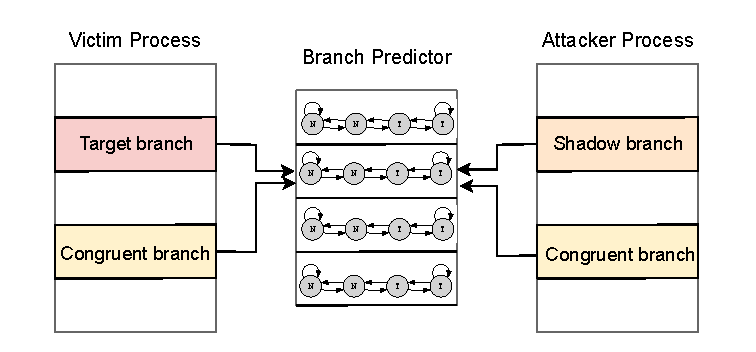
\includegraphics[width=\linewidth]{img/branch_predicator.drawio.pdf}
  \caption{分岐予測器のトレーニング}
  \label{fig:branch_predicator}
\end{figure}


攻撃者はまず、2行目の\var{if}文(Victim branch, VB)の条件が True と予測されるように分岐予測器をトレーニングする必要がある。近年のCPUにおける分岐予測器は、通常、分岐命令の仮想アドレスをインデックスとして利用する\cite{fog2016microarchitecture,8835233}。この特性を利用し、攻撃者は、Victim branchと同一の仮想アドレスを持つ分岐命令(Shadow branch)を用いて、自身のプロセス内で分岐予測器をトレーニングできる。また、仮想アドレスの一部のみが分岐予測器のインデックスとして使用される場合には、Victim branchと仮想アドレスの一部が一致する分岐命令(Congruent branch)を使用してトレーニングを行うことも可能である。これにより、攻撃者は図\ref{fig:branch_predicator}に示すように、複数の経路を通じて分岐予測器をトレーニングできる\cite{canella2019systematic}。図\ref{BCB}のコード辺では、2行目の条件分岐が True になるような入力を繰り返し与え、分岐予測器を True 側にトレーニングする。\par

次に、攻撃者は変数\var{i}に\var{array1\_size}以上の値を与える。この場合、通常の実行では2行目の境界チェックによって、3行目と4行目の処理は実行されずにプログラムは終了する。しかし、先述のトレーニングの結果、分岐予測器は分岐条件が真になると誤って予測するため、3,4行目が投機実行される。この投機実行により、3行目では攻撃者が操作可能な変数\var{i}を使用して境界外アクセスが発生する(Read Secret, RS)。読み取られた値は、4行目で\var{array2}へのアクセスのインデックスとして使用され、キャッシュの状態に変更が加えられる(Leak Secret, LS)。その後、CPUは分岐条件の評価結果から分岐予測が誤っていたことを知り、投機実行中のメモリアクセス結果を破棄するが、キャッシュの状態はパフォーマンスの観点からロールバックされない。\par

最後に、攻撃者は先述のPrime+ProbeやFlush+ReloadといったSide-Channel Attackを用いて、投機実行中のメモリアクセスで使用されたキャッシュラインを把握する。4行目で読み取られたメモリアドレスは秘密情報に依存しており、使用されるキャッシュラインの位置は仮想アドレスによって決定するため、どのキャッシュラインが使用されていたかを把握することで、秘密情報を復元することが可能になる。\par
以上のことから、Spectre-PHT脆弱性は、(i) 攻撃者が制御可能な分岐命令(VB)、(ii) 秘密情報を読み取る命令(RS)、(iii) 読み取った秘密情報をキャッシュ状態に反映させる命令(LS)の3つの命令から構成される。ただし、実際の攻撃では、VBに該当する命令の分岐予測から開始した投機実行が終了する前に、LS及びRSに該当する命令の実行を完了する必要がある。これは、キャッシュ状態に秘密情報を反映させる前に投機実行が終了してしまうと、実行状態がロールバックされ、攻撃が成立しないためである。投機実行可能な命令数はCPUのROBのサイズに制限されており(詳しくは\ref{sec:spec_exec}を参照)、投機実行可能な命令数の上限を投機ウィンドウ (SEW)という。このように、Spectre-PHTに対して脆弱なコード辺はSpectre Gadgetと呼ばれる。以降ではSpectre-PHTを単にSpectreと表記する。


\subsubsection{直列化命令}

\begin{figure}
  \begin{minted}[linenos,escapeinside=@@,label=BCB,autogobble]{c}
#include <x86intrin.h>
i = input();
if (i < array1_size) {
  _mm_lfence();   // Add lfence
  secret = array1[i];  
  tmp &= array2[secret];  
}
\end{minted}
  \caption{Spectre-PHT 脆弱性を含むコード片に対し、lfence命令による防御策を適用した例}
  \label{lfence}
\end{figure}

Spectre攻撃には投機実行が必要である。そのため、命令がその命令に至る制御フローが確定した場合にのみ実行されるようにすることで、Spectre攻撃を防御することが可能である。このアプローチとして、元のプログラムに直列化命令を挿入して修正する方法が提案されている\cite{8835233}。例えばx86アーキテクチャの場合、lfence命令を使用することが可能である。lfence命令は、全ての先行するメモリロード命令が完了するまで、後続のメモリロード命令を投機実行させないようにする制御命令である。プログラム中の全ての条件分岐命令の分岐先にlfence命令を挿入することで、それ以降のメモリロード命令の投機実行を抑制し、Spectre攻撃を防御できる。\par

図\ref{BCB}のコード片に対して lfence 命令を挿入してSpectre攻撃に対して堅牢化したコード辺を図\ref{lfence}に示す。4行目にlfence命令が挿入されることで、3行目の分岐条件の評価が終了し分岐先が確定してから、後続の配列へのアクセスが行われるようになる。\par 
しかし、CPUの分岐予測を無効化することで、大幅にパフォーマンスが低下することが知られている。既存研究\cite{wang2018oo7}では、元のプログラムの全ての条件分岐命令に対してlfence命令を挿入した場合、プログラムの実行時間が最大3.25倍程度に増加することが報告されている。

\subsubsection{Speculative Load Hardening}

\begin{figure}
  \begin{minted}[linenos,escapeinside=@@,label=BCB,autogobble]{c}
void leak(int data);
void example(int* pointer1, int* pointer2) {
  if (condition) {
    // ... lots of code ...
    leak(*pointer1);
  } else {
    // ... more code ...
    leak(*pointer2);
  }
}
\end{minted}
  \caption{SLH適用前のSpectre Gadget}
  \label{SLH_before}
\end{figure}

\begin{figure}
  \begin{minted}[linenos,escapeinside=@@,label=BCB,autogobble]{c}
uintptr_t all_ones_mask = std::numerical_limits<uintptr_t>::max();
uintptr_t all_zeros_mask = 0;
void leak(int data);
void example(int* pointer1, int* pointer2) {
  uintptr_t predicate_state = all_ones_mask;
  if (condition) {
    predicate_state = !condition ? all_zeros_mask : predicate_state;
    // ... lots of code ...
    pointer1 &= predicate_state;
    leak(*pointer1);
  } else {
    predicate_state = condition ? all_zeros_mask : predicate_state;
    // ... more code ...
    int value2 = *pointer2 & predicate_state;
    leak(value2);
  }
}
\end{minted}
  \caption{SLH適用後のコード辺}
  \label{SLH_after}
\end{figure}



Spectre攻撃に対する実行時オーバーヘッドが少ない防御策として、Carruthによって提案されたSpeculative Load Hardening(SLH)\cite{LLVM-SLH}がある。SLHはコンパイラベースの防御手法であり、分岐命令を使用せずに、メモリアクセス命令が有効な制御フローパス上で実行されているかを確認するコードを計装する。以降では、先行研究\cite{LLVM-SLH}に示されているコード例を元に、SLHの概要を説明する。\par

図\ref{SLH_before}と図\ref{SLH_after}は、それぞれSLH適用前と後のコード辺である。ここで、関数\var{leak}は投機実行された場合に引数のデータを攻撃者に漏洩させると仮定する。変数\var{predicate\_state}は、現在の実行が分岐予測ミスによる分岐先であるかを表しており、7行目と12行目において、条件\var{condition}が満たされない場合は\var{all\_zeros\_mask}(全てのビットが0の値)、満たしている場合は\var{all\_ones\_mask}(全てのビットが1の値)が代入される。重要な点として、7行目の三項演算子は分岐命令が使用されない形で機械語に変換される必要がある。これにより、7行目の条件\var{condition}が投機実行によってバイパスされないことを保証する。x86アーキテクチャでは、cmov命令を用いることで実現可能である\cite{LLVM-SLH}。\par
分岐予測が正しい場合は、var{predicate\_state}には\var{all\_ones\_mask}が格納される。そのため、9行目及び13行目で論理積が取られても、\var{pointer1}及び\var{pointer2}の値はそのまま保持される。一方、分岐予測が誤っている場合、var{predicate\_state}には\var{all\_zeros\_mask}が格納されている。これにより、論理積を取ることで、\var{pointer1}と\var{pointer2}の値は0となる。その結果、関数\var{leak}が実行されても攻撃者が意図したデータは漏洩しない。\par

lfence命令を用いた防御策では、lfence命令以降に続くすべてのメモリロード命令の投機実行が抑制される。このため、Spectre攻撃に関与しない安全なメモリロード命令であっても、投機実行が制限されてしまう。また、分岐予測が正しく行われた場合でも、lfence命令以降の投機実行が抑制されるため、パフォーマンスが大幅に低下する。一方、SLHは、投機実行による漏洩のリスクがある危険なメモリロード命令に対してのみ投機実行を抑制する。そのため、投機実行可能なメモリロード命令を増やすことができ、lfence命令と比較して小さい実行時間オーバーヘッドでSpectre攻撃を防御することができる。しかし、それでも全てのメモリロード命令をSLHで強化する場合、大規模なアプリケーションでは実行時オーバーヘッドが30\%程度になることが報告されている\cite{LLVM-SLH}。

\subsection{Spectre Gadgetの検出}
Spectre攻撃に対してプログラムを堅牢化するために、lfence命令やSLHを全ての条件分岐命令やメモリロード命令に適用する場合、大きな実行時オーバーヘッドが発生する。そこで、プログラム内の潜在的なSpectre gadgetを見つけ、これらのgagetのみに防御策を適用して、実行時オーバーヘッドを軽減する方法が提案されている。\par

Spectre Gadgetを検出するためのプログラム解析手法は大きく分けて、静的解析\cite{Spectre-Scanner,wang2018oo7,guarnieri2020spectector,wang2020kleespectre}による手法と、動的解析\cite{oleksenko2020specfuzz,qi2021spectaint,johannesmeyer2022kasper}による手法の2種類に分類される。投機実行はハードウェアによる機能であるため、これらの解析手法の大半がソフトウェアレベルで投機実行をシミュレートすることでSpectre gadgetを検出している。以降では、それぞれの手法がどのように投機実行をシミュレートし、Spectre gadgetを検出しているかを説明する。その代表例として、静的解析による検出手法としてKLEESpectre\cite{wang2020kleespectre}を、動的解析による検出手法としてSpecFuzz\cite{oleksenko2020specfuzz}を紹介する。これらの既存手法は本研究における実装の基盤にもなっているため詳しく説明する。

\subsubsection{KLEESpectre}

\begin{figure}
  \begin{minted}[linenos,escapeinside=@@,label=BCB,autogobble]{c}
    uint32_t SIZE = 16;
    uint8_t array1[16], array2[256*64], array3[16];

    uint8_t foo(uint32_t x) {
      uint8_t temp = 0;
      if(x < size) {    // b1
        // A
        temp = array1[x]; 
        temp |= array2[temp];
        if(x <= 8) {  // b2
          // B 
          temp |= array2[8];
        }
      }
      // C
      temp |= array3[8]
      return temp;
    }
\end{minted}
  \caption{KLEESpectreにおけるコード例}
  \label{klee_code}
\end{figure}

KLEESpectre\cite{wang2020kleespectre}は記号実行により、プログラム中のSpectre gadgetを検出するツールである。記号実行とは、プログラムに具体的な値ではなく、記号的な変数を入力として与えることで、プログラムの全ての実行パスを網羅的に解析する静的手法である。入力を記号化することで、プログラムが異なる入力で取る可能性のある複数のパスを同時に探索することができる。記号実行は記号実行エンジンによって行われ、探索された制御フローパスごとに、(i) そのパスに沿って実行された分岐によって満たされる条件を記述するパス制約、および (ii) 各変数を記号式または具体的な値にマップする記号的なメモリ状態を保持することで現在の実行状態を管理する\cite{baldoni2018survey}。\par

KLEESpectreは記号実行エンジンであるKLEE\cite{cadar2008klee}をSpectre gadgetの検出用に拡張したものであり、単純なパターンマッチングによる手法\cite{Spectre-Scanner}と比較して高い精度でSpectre gadgetを検出することができる。\par
まず、\cite{wang2020kleespectre}に挙げられるコード辺を用いて、KLEESpectreがどのように分岐予測による投機実行をシミュレートしているかを説明する。図\ref{klee_code}は典型的なSpectre脆弱性を含んでいるコード辺である。分岐\var{b1}が誤って分岐予測された場合、\var{x}の値は\var{SIZE}以上となるので、8行目で境界外アクセスが発生し、秘密情報が\var{temp}に読み取られる可能性がある。その後、9行目で\var{temp}が\var{array2}へのアクセスのインデックスとして使用されることで、秘密情報がキャッシュの状態として漏洩する。\par
通常の記号実行の場合、条件分岐命令に遭遇すると、分岐条件が満たし、Taken側の基本ブロックに進んだ記号状態と、分岐条件を満たさず、Not taken側の基本ブロックに進んだ記号状態の2つの状態が新しく生成される。しかし、KLEESpectreでは投機実行をシミュレートするため、上記の2つの状態に加え、分岐条件が満たし、Not taken側の基本ブロックに進んだ記号状態と、分岐条件を満たさず、Taken側の基本ブロックに進んだ記号状態の2つの状態も生成される。\par
例えば、KLEESpectreが図\ref{klee_code}の分岐\var{b1}に遭遇した場合、以下の4つの状態が新しく生成される。\par

\begin{enumerate}[label=(\arabic*)]
  \item \var{x < SIZE} を満たし、分岐\var{b1}が正しく分岐予測された状態
  \item \var{x < SIZE} を満たさず、分岐\var{b1}が正しく分岐予測された状態
  \item \var{x < SIZE} を満たし、分岐\var{b1}が誤って分岐予測された状態
  \item \var{x < SIZE} を満たさず、分岐\var{b1}が誤って分岐予測された状態
\end{enumerate}

\begin{figure}[tb]
  \centering
  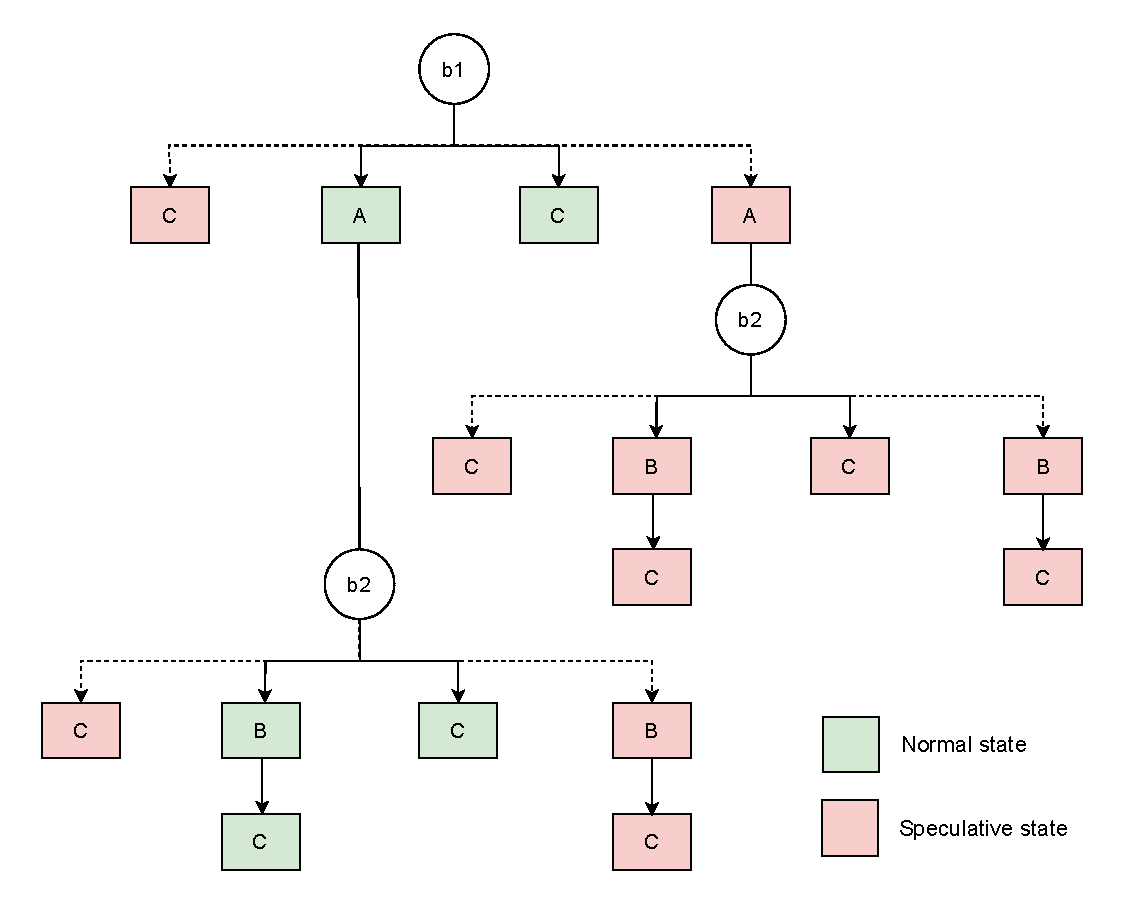
\includegraphics[width=\linewidth]{img/klee_CFG.drawio.pdf}
  \caption{投機的なパスを含んだ制御フローグラフ}
  \label{fig:klee_cfg}
\end{figure}


(1)の場合、KLEESpectreは現在の記号状態のパス制約に\var{x < SIZE}を追加し、基本ブロック\var{A}に移動し、実行を続ける。
(2)の場合も同様に、現在の記号状態のパス制約に\var{x >= SIZE}を追加し、基本ブロック\var{C}に移動し、実行を続ける。
(3)の場合、KLEESpectreは現在の記号状態のパス制約に\var{x < SIZE}を追加するが、分岐予測ミスにより、基本ブロック\var{C}に移動し、実行を続ける。
(4)の場合も同様に、現在の記号状態のパス制約に\var{x >= SIZE}を追加するが、分岐予測ミスにより、基本ブロック\var{A}に移動し、実行を続ける。このようにKLEESpectreは分岐予測ミスによる投機的なパスも考慮して記号実行を行うようにKLEEを拡張している。図\ref{fig:klee_cfg}において、投機的なパスも含めた図\ref{klee_code}の制御フローグラフを示す。\par
図\ref{fig:klee_cfg}では、実線が直前の分岐命令が正しく分岐予測された場合のパスを、点線が直前の分岐命令が誤って分岐予測された場合の投機的パスを表している。緑色の基本ブロックは通常の実行パスにおける基本ブロックを、赤色の基本ブロックは投機的なパスにおける基本ブロックを表している。KLEESpectreは全ての分岐命令が攻撃者によって訓練されていると仮定し、投機実行のシミュレートを行う。このシミュレーションにおいて、投機的な状態が以下のいずれかの条件を満たした場合、CPUにおける投機実行の終了動作を再現するためにその記号状態を破棄する。\par
\begin{itemize}
  \item 投機的なパス上で実行した命令数が投機ウィンドウの制限に達した場合
  \item 直列化命令に遭遇した場合
  \item 例外が発生した場合
\end{itemize}

また、本研究のテーマと関連する重要な点として、KLEESpectreでは投機実行をネストしてシミュレートする場合がある。図\ref{klee_code}では、分岐\var{b1}の分岐予測ミスによる投機実行中に分岐\var{b2}に遭遇した場合、KLEESpectreは重ねて分岐\var{b2}の分岐予測ミスをシミュレートする。このように、KLEESpectreでは、ある分岐命令の分岐予測ミスから開始された投機実行中に、別の分岐命令に遭遇した場合、重ねて投機実行をシミュレートする。実際のCPUにおいても、このようなネストされた投機実行は可能であり\cite{mambretti2019speculator}、KLEESpectreは正しくCPUの投機実行をシミュレートしていると言える。\par
次に、KLEESpectreがどのようにSpectre Gadgetを検出するかについて説明する。
まず、投機的に実行されたパスにおけるメモリアクセスを監視し、それらが秘密情報を参照している場合、その命令をRS(Read Secret)として記録する。KLEESpectreでは、投機的パスにおいて攻撃者が操作可能な値(記号変数)をアドレスとして使用した境界外のメモリアクセスは、すべて秘密情報を参照していると仮定し、保守的な解析を行っている。境界外のメモリアクセスはKLEEに組み込まれているチェック機構を利用して、識別している。次に、秘密情報に依存する値を用いてメモリアクセスが行われた場合、その命令をLS(Leak Secret)として記録する。LSが検出されると、直前に分岐予測ミスが発生した分岐命令と、RSおよびLSに該当する命令のセットをまとめて、Spectre Gadgetとして記録する。\par

KLEESpectreは記号実行を活用することで、単純な静的解析手法や動的解析手法に比べて、プログラムの網羅的な解析が可能である。これにより、より高い精度でSpectre gadgetを検出できる。しかし、大規模なコードや探索すべきパスが多い複雑なプログラムに対しては、スケールしないという課題がある。\par

\subsubsection{SpecFuzz}

\begin{figure}[tb]
  \centering
  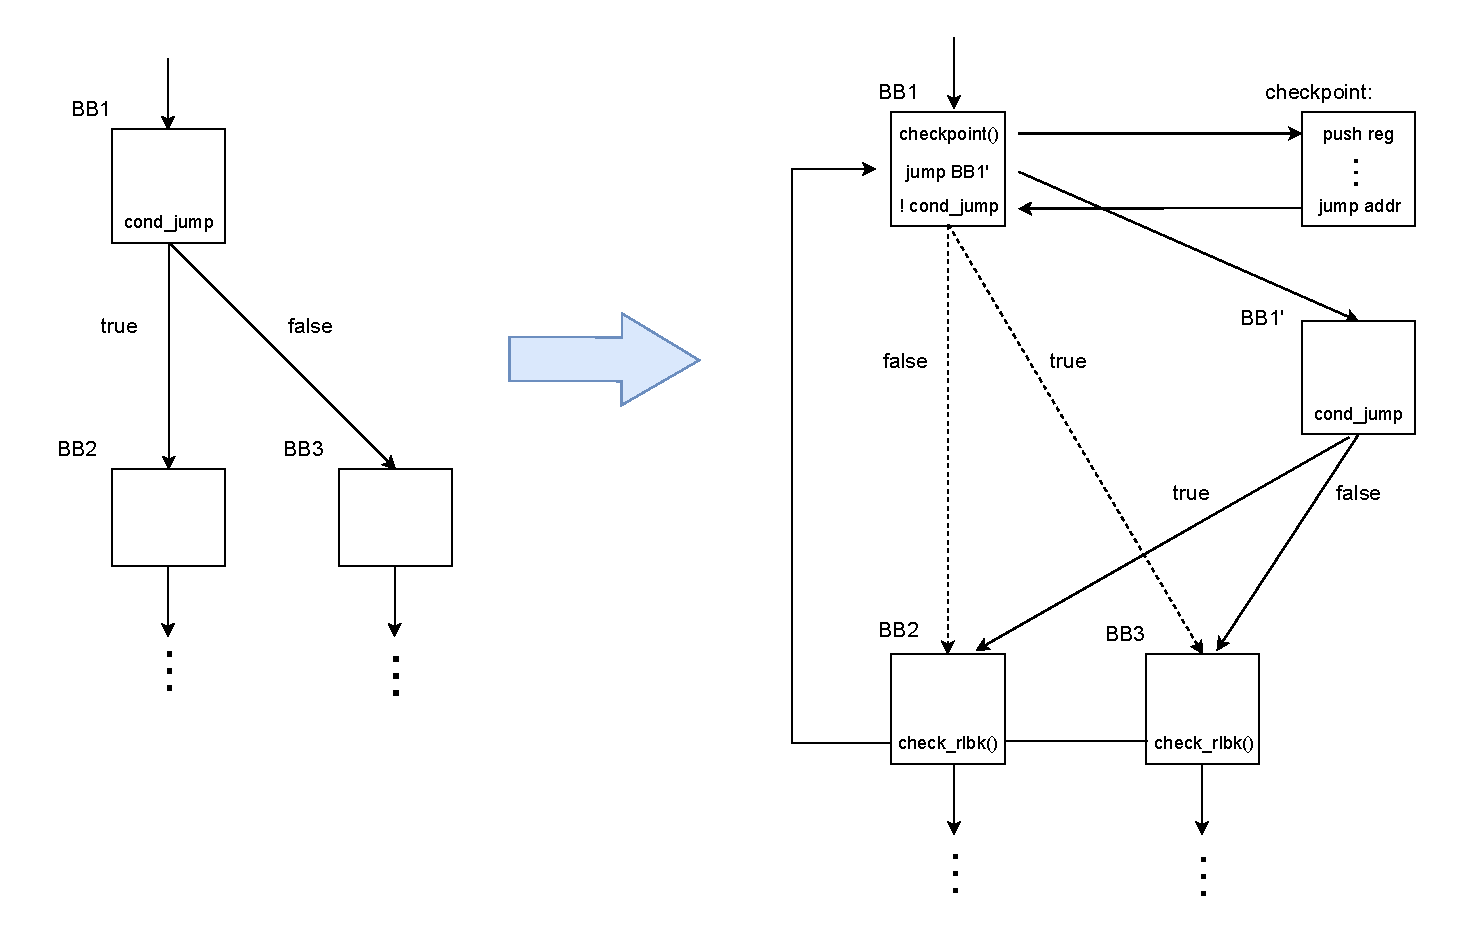
\includegraphics[width=\linewidth]{img/specfuzz_instrument.drawio.pdf}
  \caption{SpecFuzzによる計装前と計装後の制御フローグラフの概略}
  \label{fig:specfuzz_instrument}
\end{figure}


SpecFuzz\cite{oleksenko2020specfuzz}は、ファジングを利用してプログラム内のSpectre Gadgetを検出するためのツールである。ファジングとは、プログラムにランダムに生成された入力を与えることで、バグや脆弱性を検出する動的解析手法である。ファザーは、文法に基づいてゼロからランダムな入力を生成するか、既存の入力コーパスを変更して新たな入力を作成する。これらの生成された入力をプログラムに与え、その挙動を監視することで、未知のバグや脆弱性を特定する。また、ファジングの重要なパラメーターの 1 つにカバレッジがある。これは、ファジング中にプログラムがどの程度広範囲にテストされたかを示している。一般的には、ファジング中に少なくとも 1 回実行された制御フローグラフのエッジ数とプログラム内のエッジの合計数の比率として定義される。当然カバレッジが低いと検出対象の見逃しが発生するため、カバレッジを向上させることが多くのファザーにとって重要である。\par
まず、SpecFuzzがどのように分岐予測による投機実行をシミュレートしているかを説明する。SpecFuzzは、テスト対象のプログラムに対してx86アーキテクチャ用のLLVMコンパイラバックエンドパスを利用し、投機実行のシミュレーションに必要なコードを計装する。図\ref{fig:specfuzz_instrument}に計装前のプログラムの制御フローグラフとSpecFuzzによる計装後の制御フローグラフの概略図を示す。点線が分岐予測ミスによるパス、実線が通常の実行によるパスを表している。
また、KLEESpectreと同様に、全ての分岐命令が攻撃者によってトレーニングされていると仮定し、投機実行をシミュレートする。\par
SpecFuzzでは、まず全ての条件分岐命令の直前にチェックポイントを配置する関数(\var{specfuzz\_chkp})の呼び出しを計装する。この関数は、投機実行のシミュレーション開始地点を示し、シミュレーション終了後に通常の実行パスへ戻るため、現在のCPU状態を保持する役割を持つ。具体的には、以下の情報をスナップショットとして取得し、メモリに保存する。\par

\begin{itemize}
  \item レジスタ値(GPR、フラグ、SIMD、浮動小数点レジスタなど)
  \item ロールバック先のアドレス
  \item メタデータ (スタックポインタ、シミュレーション中に実行した命令数など)
\end{itemize}

次に、全ての分岐命令(\var{cond\_jump})を、その分岐条件を反転させた命令(\var{!cond\_jump})に置き換える。この操作により、分岐命令に遭遇するたびに通常の実行パスとは逆方向に処理が進み、投機実行のシミュレーションが開始する。さらに、メモリを変更する全ての命令(mov, push, callなど)の直前には、変更対象のアドレスとその直前の値を記録するコードを挿入する。これにより、投機実行のシミュレーション中に行われた全てのメモリの変更がログに記録され、ロールバック時にシミュレーション開始時点の状態に戻すことが可能になる。\par
投機実行のシミュレーションは、Machine IR (MIR)レベルで実行された命令数が投機ウィンドウによる上限に達するか、直列化命令に遭遇した場合に終了する。各基本ブロックの最後では、シミュレーション中に実行された命令数が投機ウィンドウに達しているかをチェックし、上限に達していない場合、シミュレーションを継続する。上限に達していた場合、シミュレーションを終了するため、ロールバック用の関数(\var{specfuzz\_rlbk})が呼び出され、直前のチェックポイント地点にシャンプし、スナップショットに基づいてレジスタやメモリの状態を復元した後、正しい実行パスを再開する。\par
次に、SpecFuzzがどのようにSpectre Gadgetを検出するかについて説明する。SpecFuzzは、投機実行のシミュレーション中に境界外アクセスが検出された場合、その直前に分岐予測ミスが発生した分岐命令と、境界外アクセスが行われた命令を合わせてSpectre gadgetとして報告する。境界外アクセスの検出には、AddressSanitizer(ASan)\cite{serebryany2012addresssanitizer}が使用される。\par
この手法は境界外アクセスが攻撃者の操作している値に依存しているかや、境界外アクセスで読み取った値がキャッシュへ転送されるか(LSが存在するか)といったことは考慮されておらず、単純な検出手法である。そのため、実際には攻撃に利用できないgadgetも多数検出される可能性がある\cite{qi2021spectaint}。しかし、単純化された検出機構により他のファジングベースのSpectre gadgetの検出手法\cite{qi2021spectaint,johannesmeyer2022kasper}と比較して、より高いファジングスループットを実現できる。\par

SpecFuzzはファジングを活用することで、記号実行を用いた手法と比較して大規模なプログラムに対してもスケールする。しかし、ファジングのカバレッジ不足により、一部のSpectre gadgetを見逃す可能性がある。また、検出機構が単純化されているため、実際には攻撃に利用できないgadgetが誤って検出される可能性もある。


%%%%%%%%%%%%%%%%%%%%%%%%%%%%%%%%%%%%%%%%%%%%%%%%%%
%% 問題設定
%%%%%%%%%%%%%%%%%%%%%%%%%%%%%%%%%%%%%%%%%%%%%%%%%%
\section{問題設定}
本論文では、スケーラビリティと精度を両立するSpectre Gadgetの検出手法を提案する。Spectre Gadgetを正確かつ効率的に検出することは、最低限の実行時オーバーヘッドでプログラムをSpectre攻撃に対して堅牢化するために不可欠である。以降では、まず既存のSpectre Gadgetの検出手法が抱える問題点について述べる。その後、その問題点を示すMotivating Exampleを提示し、本研究の目的を明確化する。

\subsection{既存手法の問題点}

\subsubsection{記号実行}

\begin{figure}
  \begin{minted}[linenos,escapeinside=@@,label=BCB,autogobble]{c}
    int i;
    symbolic_var(i); // Symbolize variable i
    while(i > 0) {
      ...
      i--;
    }
\end{minted}
  \caption{記号実行におけるパス爆発}
  \label{path_explosion}
\end{figure}



記号実行を用いたSpectre Gadgetの検出手法\cite{guarnieri2020spectector,wang2020kleespectre}の問題点は、大規模なプログラムに対してスケールしないという点である。これは一般的な記号実行による解析に共通する問題でもあるが、Spectre Gadgetの検出ツールは通常のパスに加えて、投機的なパスも考慮する必要があるため、これはより顕著な問題となる。この問題の主な原因はパス爆発とストア状態の爆発として知られている\cite{baldoni2018survey}。\par

パス爆発とは、プログラム内の分岐数に比例して探索すべき実行パスが指数関数的に増加する現象を指す。記号実行エンジンは、分岐箇所に遭遇すると現在の状態を分岐方向ごとに分割し、新たな状態を生成する。このため、分岐が多いプログラムでは実行パスの数が急激に増加し、解析時間やメモリ使用量が膨大となる。結果として、すべての実行パスを網羅的に解析することが現実的に不可能となる場合がある。\par

パス爆発の主な原因の一つは、ループ構造に起因するものである。ループは分岐命令として扱われるため、各反復ごとに分岐方向に対応する新しい状態が生成される。さらに、図\ref{path_explosion}に示すように、ループ条件に記号化された変数が含まれる場合、ループの反復回数が具体的に決定できず、最大のループ回数を想定して解析が行われる可能性がある。一般的なツールでは、ループの解析を限られた回数に制限しているが、この場合、検出対象を見逃す可能性もある。\par

\begin{figure}
  \begin{minted}[linenos,escapeinside=@@,label=BCB,autogobble]{c}
    size_t i, j;
    int temp;
    symbolic_var(i); // Symbolize variable i
    symbolic_var(j); // Symbolize variable j
    int array[5] = {0};
    if(i < 5 && j < 5) {
      array[i] = 1;
      temp = array[j];
    }
\end{minted}
  \caption{記号実行におけるストア状態の爆発}
  \label{store_explosion}
\end{figure}


ストア状態の爆発とは、記号実行において抽象的に扱われるメモリ状態の数が急激に増加する現象を指す。記号実行エンジンは、プログラムのメモリ操作を正確にモデル化するために、各メモリアドレスを具体的な値または記号式に関連付けたストア状態というデータ構造を保持する。そのため、記号化されたアドレスに対して読み取りや書き込みが行われる場合、操作の結果として生じる可能性のある全てのストア状態を考慮する必要がある。その結果、新しいストア状態が次々に生成され、ストア状態の数が急激に増加する。この現象は、大規模なプログラムや複雑なメモリアクセスパターンを持つコードにおいて特に顕著である。\par

図\ref{store_explosion}に示すコード例を用いて、ストア状態の爆発について具体的に説明する。このコードでは、変数\var{i}と\var{j}が記号化されている。まず、7行目の配列への書き込みに注目する。この箇所では、\var{i}が記号化されているため、\var{array[0]}から\var{array[4]}のいずれかの要素が1に書き換えられる可能性がある。その結果、これら5つの可能性を全て考慮するため、7行目の実行後に現在の状態から5つの新しい状態が分岐される。
同様に、8行目の配列への読み取りにおいても、\var{j}が記号化されているため、\var{array[0]}から\var{array[4]}のいずれかの要素が読み取られ、変数\var{temp}に格納される。この場合も、5つの可能性を考慮するため、8行目の実行後にさらに5つの新しい状態が分岐し、最終的には最初の状態から新しく25個の状態に分岐することになる。\par
この例では、変数\var{i},\var{j}の範囲が制限されていたため、メモリ操作が参照する可能性のあるアドレスのセットは比較的小さかったが、一般的には、記号化されたアドレスはメモリ内の任意のアドレスを参照する可能性があるため、ストア状態の数が爆発的に増加する可能性がある。\par
パス爆発とストア状態の爆発の問題は、記号実行を用いてSpectre Gadgetを検出する場合により顕著になる。これは、分岐予測ミスによる投機的なパスを考慮することで、通常の記号実行に比べて探索すべきパス数が大幅に増加するからである。通常の実行パス上の状態と異なり、投機的なパス上の状態は投機ウィンドウの上限に達した時点で破棄されるため最後まで残ることはない。しかし、それでも解析時間や最大メモリ使用量に大きな影響を与えるため、大規模なプログラムや複雑な制御フローを持つプログラムに対してはスケールしない。\par

\subsubsection{ファジング}
ファジングを用いたSpectre Gadgetの検出手法における主な問題点は、カバレッジ不足によりGadgetの見逃しが発生する可能性がある点である。ファジングは記号実行とは異なり、生成された入力によって実行されたパス上に存在するGadgetしか検出できない。これは一般的なファジングツールに共通する問題でもある。\par
さらに、ファザーが脆弱性を引き起こす入力を生成しない場合、Spectre Gadgetを検出することはできない。例えば、図\ref{BCB}に示すコードを考える。ここで、ファザーが条件\var{i < array1\_size}を満たす入力\var{i}を生成した場合、3行目および4行目は通常実行される。そのため当然、3行目で境界外アクセスが発生しないので、脆弱性は検出されない。一方、\var{i < array1\_size}を満たさない入力\var{i}を生成することで、3行目及び4行目が投機実行がシミュレートされ、3行目の境界外アクセスが引き起こされ、初めて脆弱性を検出できる。このように、ファジングによるSpectre Gadgetの検出は、通常の実行パスだけでなく、投機的なパスも漏れなくテストすることが必要である。\par

\subsection{Motivating Example}
\label{sec:MotivatingExample}

\begin{figure}
  \begin{minted}[linenos,escapeinside=@@,label=BCB,autogobble]{c}
#define ARRAY1_SIZE 16
uint8_t array1[16] = {1, 2, 3, 4, 5, 6, 7, 8, 9, 10, 11, 12, 13, 14, 15, 16};
uint8_t array2[256 * 512];
uint8_t temp = 0;

void var(size_t index) {
    if (index < ARRAY1_SIZE / 2) {   // b2
        // C
        temp &= array2[array1[index] * 512];
        if (index < ARRAY1_SIZE / 4) {  // b3
            // D
            temp &= array2[array1[index] * 512];
        }
    }
    // E
}

void foo(size_t index) {
  while (index < ARRAY1_SIZE) {  // b1
    // A
    temp &= array2[array1[index] * 512];
    var(index);
    ++index;
  }
    // B
}

int main() {
  size_t num = input();
  foo(num);
  return 0;
}
   \end{minted}
  \caption{Motivating Example}
  \label{MotivatingExample}
\end{figure}

図\ref{MotivatingExample}は、記号実行を用いたSpectre Gadgetの検出において、投機的な状態数が爆発する具体例を示している。この図には、3つのSpectre Gadgetが含まれている。1つ目は、18行目が分岐予測ミスされた後に実行される9行目の命令である。2つ目は、9行目と18行目の両方が分岐予測ミスされた後に実行される10行目の命令である。そして3つ目は、18行目、9行目、11行目の全てが分岐予測ミスされた後に実行される12行目の命令である。先述の通り、CPUはネストされた投機実行が可能であり、既存の記号実行による手法\cite{guarnieri2020spectector,wang2020kleespectre}では、これらのGadgetを漏れなく検出するため、ネストされた分岐予測ミスをシミュレートする必要がある。そのため、投機ウィンドウの上限に達するまで、分岐命令に遭遇するたびに以下の4つの新たな状態が生成され、状態数の爆発に大きく寄与していると考えられる。\par

\begin{itemize}
  \item 分岐条件を満たし、Taken側へ遷移した状態
  \item 分岐条件を満たさず、Not taken側へ遷移した状態
  \item 分岐条件を満たさず、分岐予測ミスによりTaken側へ遷移した状態  
  \item 分岐条件を満たし、分岐予測ミスによりNot taken側へ遷移した状態
\end{itemize}

しかし、既存研究\cite{oleksenko2020specfuzz}では、現実世界の検体において、10行目や12行目のような、ネストされた分岐予測ミスによりトリガーされるGadgetは少ないことが報告されている。この直感的な理由として、多くのメモリアクセス命令は、単一の境界チェック条件で保護されており、10行目や12行目のような複数の境界チェックで保護されているメモリアクセス命令は稀であるからと考えられる。また、複数の分岐命令を訓練することは、攻撃者にとって非常に困難であるため、このようなGadgetが実際の攻撃で利用される可能性は低いと考えられる。\par
既存の記号実行による手法では、Gadgetが検出される可能性の低い(あるいは、検出しても攻撃に利用されにくい)ネストされた分岐予測ミスにより到達する投機的な状態まで探索しているため、スケーラビリティが低下していると考える。\par

表\ref{klee_test}に図\ref{MotivatingExample}をKLEESpectreで解析を行った結果を示す。実験環境及び構成は6.3節の通りである。表\ref{klee_test}からわかる通り、小規模な検体でありながら、通常実行において探索した状態数(State)に比べて、非常に多くの投機的な状態(Speculative states)を探索している。これにより、通常の記号実行による解析と比較して解析時間と最大メモリ使用量が大幅に増加し、スケーラビリティが低下していると考える。\par

\begin{table}[h]
  \centering
  \caption{KLEESpectreによるMotivating Exampleの解析結果}
  \label{klee_test}
  \begin{tabular}{ccccc}
    \toprule
    \textbf{Detected gadgets} & \textbf{States} & \textbf{Speculative states} & \textbf{\shortstack{Analysis Time\\(h:m:s)}} & \textbf{\shortstack{Max\\Memory Usage (KB)}}  \\
    \midrule
    3         & 17                       & 38039       &  0:0:21 &      66968     \\
    \bottomrule
  \end{tabular}
\end{table}



%%%%%%%%%%%%%%%%%%%%%%%%%%%%%%%%%%%%%%%%%%%%%%%%%%
%% 提案手法
%%%%%%%%%%%%%%%%%%%%%%%%%%%%%%%%%%%%%%%%%%%%%%%%%%
\section{提案手法}
本研究では、記号実行とファジングの解析手法を組み合わせることで、スケーラビリティと精度の両立を目指すSpectre gadget検出手法を提案する。記号実行とファジングにはそれぞれ利点と欠点が存在するが、これらを組み合わせることで、両者の欠点を補完し、スケーラビリティと精度を両立できるのではないかと考える。提案手法は、記号実行フェーズとファジングフェーズの2つのフェーズで構成され、それぞれのフェーズで検出されたgadgetを合わせて、最終的な検出結果として報告する。記号実行フェーズでは、ネストされた分岐予測を制限することで、投機的状態の探索範囲を縮小し、解析のスケーラビリティを向上させる。ファジングフェーズでは、記号実行フェーズで探索されなかった投機的な状態を集中的にテストすることで、記号実行で見逃されたgadgetを効率的に検出することを目指す。\par
以下では、記号実行フェーズとファジングフェーズのそれぞれについて、提案手法の詳細を説明する。

\subsection{記号実行フェーズ}
\subsubsection{ネストされた分岐予測の制限}
記号実行フェーズでは、ネストされた分岐予測を制限することでスケーラビリティの向上を図る。提案手法の記号実行フェーズがどのように投機実行をシミュレートするかについて、図\ref{MotivatingExample}の制御フローグラフの一部である図\ref{fig:SpecOrder_cfg}を用いて説明する。点線が分岐予測ミス、実線が通常の実行パスを表す。\par
まず、既存手法と同様に、解析が分岐\var{b1}に到達すると、投機実行のシミュレーションが開始され、以下の4つの状態に分岐する。\par

\begin{enumerate}
  \item 分岐\var{b1}の条件を満たし、Aに遷移した状態
  \item 分岐\var{b1}の条件を満たさず、Bに遷移した状態
  \item 分岐\var{b1}の条件を満たさず、分岐予測ミスによりAに遷移した状態
  \item 分岐\var{b1}の条件を満たし、分岐予測ミスによりBに遷移した状態
\end{enumerate}

これらのうち、3番目の状態のみが23行目の脆弱性を引き起こし、Spectre gadgetとして検出される。この状態から解析を進めていくと、次に分岐\var{b2}に遭遇する。既存手法では、ネストされた投機実行をシミュレートするため、\var{b2}でも分岐予測ミスを含めた4つの状態に分岐する。一方、提案手法ではネストされた分岐予測を制限し、\var{b2}における分岐予測ミスによる投機的な状態は探索しない。そのため、この状態において、以降は、投機ウィンドウの上限に達するか、直列化命令に遭遇するまで、正しい分岐方向の状態のみを探索し続ける。\par

その結果、11行目と14行目の脆弱性を引き起こすgadgetが見逃されてしまう。しかし、先述の通り、ネストされた分岐予測ミスにより引き起こされるされるgadgetは稀であるため、影響は少ないと考える。また、このようなネストされた分岐予測ミスにより到達する投機的な状態は、後述するファジングフェーズで探索を行うことで、False nagativeを最小限に抑え、精度を担保できると考える。\par

\begin{figure}[tb]
  \centering
  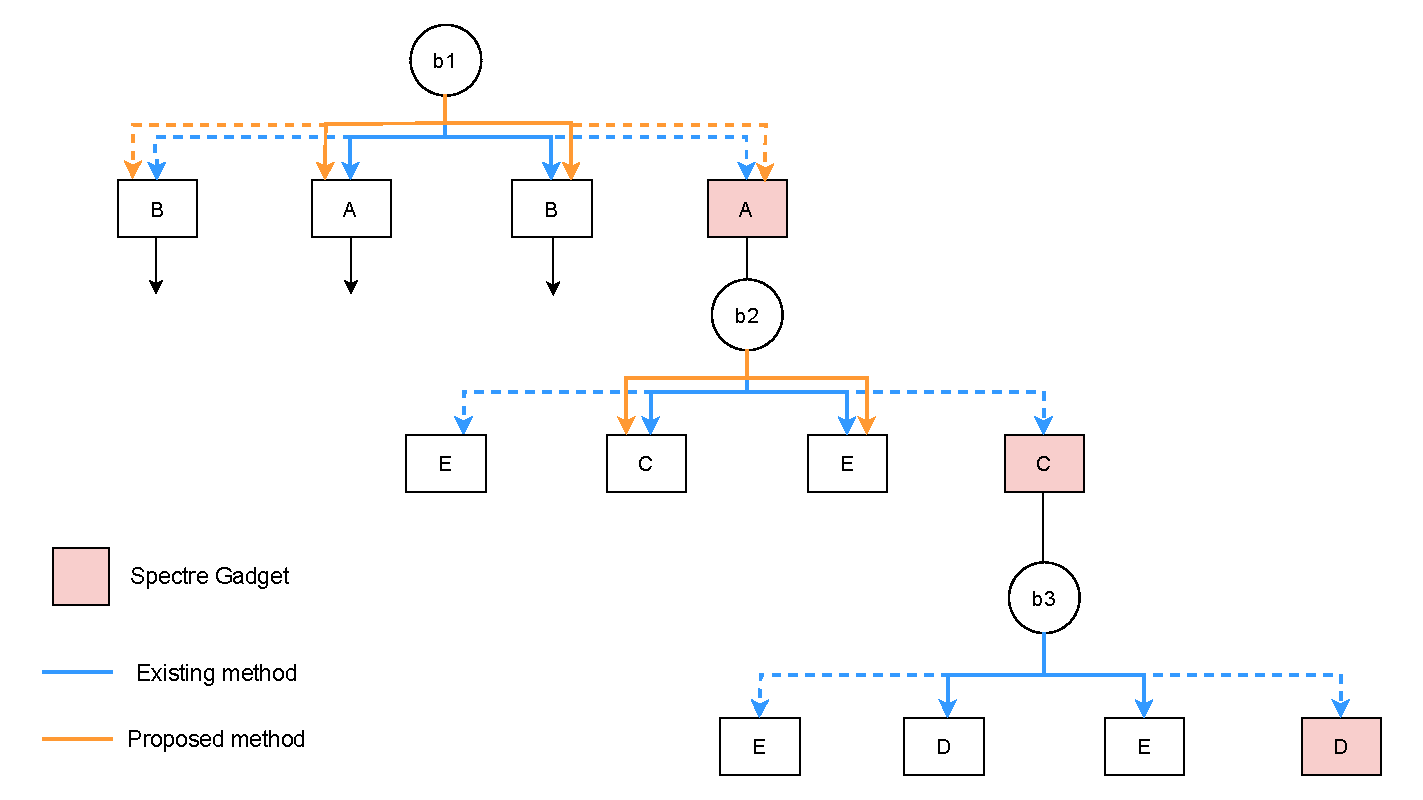
\includegraphics[width=\linewidth]{img/SpecOrder_cfg.drawio.pdf}
  \caption{ネストされた分岐予測ミスの制限}\label{fig:SpecOrder_cfg}
\end{figure}

\subsubsection{不要な分岐予測ミスの特定}
記号実行で探索されなかったネストされた分岐予測ミスにより到達する投機的な状態はファジングフェーズで探索を行う。この際、記号実行で探索した投機的な状態を再度、ファザーで探索するのは非効率的である。そこで、記号実行の過程で、分岐予測ミスをシミュレートしても、シミュレーションが終了するまでに別の分岐命令に到達できない分岐方向を特定する。その情報をファザーに提供し、それらの分岐方向への分岐予測ミスのシミュレーションを抑制することで、ファジングのスループットを向上させる。\par
図\ref{}に示すコード例を用いて具体的に説明する。


\subsubsection{目的状態までの実行トレースの取得}
\subsection{ファジングフェーズ}
\subsubsection{不要な分岐予測の抑止}
\subsubsection{スコアによるシードのスケジューリング}


%%%%%%%%%%%%%%%%%%%%%%%%%%%%%%%%%%%%%%%%%%%%%%%%%%
%% 実装
%%%%%%%%%%%%%%%%%%%%%%%%%%%%%%%%%%%%%%%%%%%%%%%%%%
\section{実装}

\begin{figure}[tb]
  \centering
  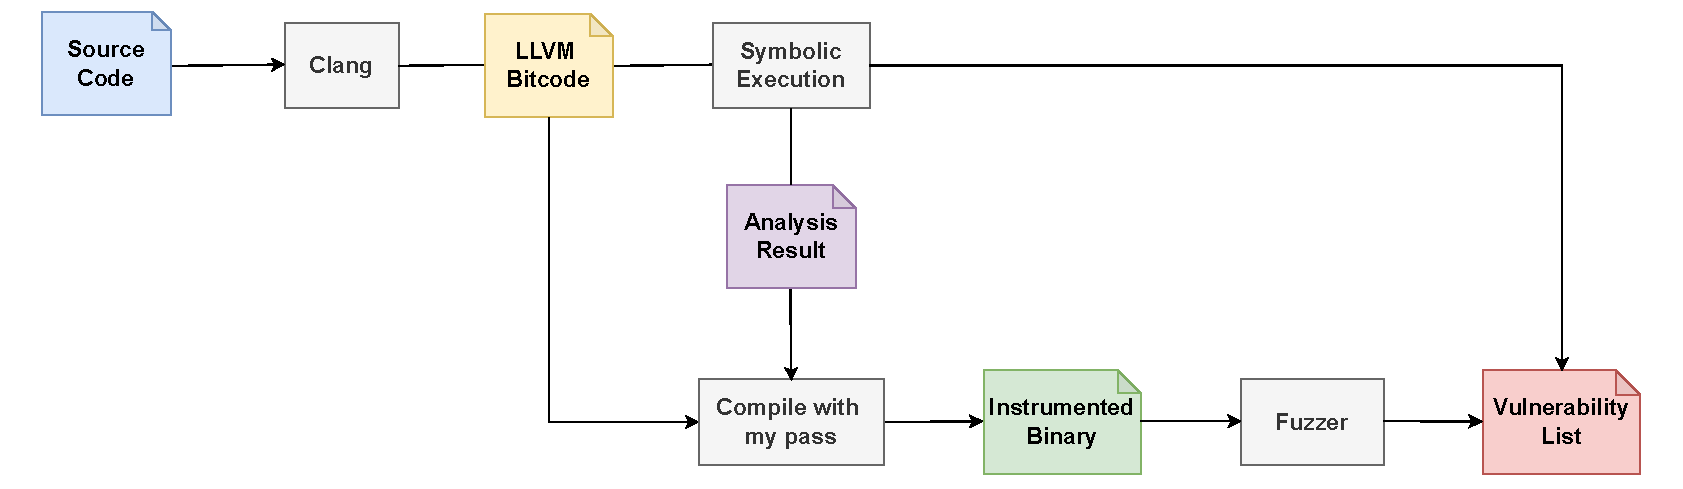
\includegraphics[width=\linewidth]{img/overall.drawio.pdf}
  \caption{提案手法の全体像}\label{fig:overall}
\end{figure}

提案手法の全体像を図\ref{fig:overall}に示す。提案手法では、記号実行をKLEESpectreを元に、ファザーをSpecFuzzを元に実装した。記号実行フェーズでは、LLVM IRを対象にOrderによる制限を加えた記号実行を行い、解析結果をファジングフェーズに提供する。ファジングフェーズでは、LLVM MIRレベルのPassを用いて、分岐予測ミスのシミュレーション用の計装と、記号実行フェーズで得られた解析結果に基づく計装を施したバイナリを生成する。この計装済みのバイナリを、カバレッジ駆動型のファジングツールであるhonggfuzz\cite{Honggfuzz}を使用してファジングを行う。スコアに基づくシードのスケジューリングは、honggfuzzを拡張することで実現している。以降では、提案手法の詳細な実装について詳しく説明する。\par

\subsection{記号実行フェーズ}
\subsubsection{Orderによる分岐予測ミスの制限}
Order値は、ユーザがコマンドラインオプションを通じて設定可能であり、デフォルト値は1に設定されている。記号実行における状態を表現するデータ構造に、現在のネストされた分岐予測ミスの回数を追跡するためのメンバ変数\var{specBranchCount}を追加し、新たな投機的状態がフォークされるたびに、\var{specBranchCount}をインクリメントする。また、投機的な状態をフォークする前に、現在の状態における\var{specBranchCount}が設定されたOrder値を超えていないかを確認する。Order値を超えていない場合は通常通りフォーク処理が行われるが、超えている場合はフォーク処理を行わず、投機的な状態の生成を抑制する。\par

\subsubsection{異常終了した投機的な状態の扱い}
記号実行では、いくつかの要因により投機的な状態が正常に終了しない場合がある。たとえば、ユーザが指定したメモリ使用量の上限やスタック数の上限に達した場合、一部の状態の探索が途中で打ち切られることがある。記号実行フェーズでRemovable Directionを特定する際、このような理由で探索が途中で終了し、ターゲット状態に到達できなかった場合、解析が継続していれば到達可能だったかどうかを判断することができない。そのため、このようなケースではその分岐予測ミスによりターゲット状態に到達する可能性があると保守的に判断し、Removable Directionではないと記録する。逆にRemovable Directionとして記録される可能性があるのは、投機的な状態が正常に終了した場合のみである。正常に終了したと判断されるのは以下のいずれかの場合のみである。\par

\begin{itemize}
  \item 投機ウィンドウの上限に達した場合
  \item 直列化命令に遭遇した場合
  \item プログラムが終了した場合
\end{itemize}

\subsection{ファジングフェーズ}
\subsubsection{分岐予測ミスの抑制を行う計装}
Removable Directionの分岐予測ミスのシミュレーションを抑制するための計装を行うアルゴリズムをAlgorithm\ref{alg:suppress_misspredication}に示す。まず各基本ブロックの終端命令を確認し、それが分岐命令であるかを調べる。分岐命令である場合、記号実行の解析結果\ref{Unnecessary_branch_result}内に該当する分岐命令が存在するかを確認する。この確認は、分岐命令の位置情報(\var{location})が一致するかどうかで行う。Removable Directionであると判断されている場合(\var{truePath}または\var{falsePath}が\var{true}である場合)、該当分岐方向の遷移先となる基本ブロックの先頭に、ランタイム関数\var{force\_rlbk}の呼び出しを挿入する。ランタイム関数\var{force\_rlbk}は、直前の分岐命令が分岐予測ミスされていた場合、シミュレーションを終了させ、即座にロールバックさせる。この計装により、Removable Directionの分岐予測ミスが発生した場合でも、即座にシミュレーションを終了させることができる。\par

\begin{algorithm}
\caption{Removable Directionの分岐予測ミスの抑制のための計装を行うアルゴリズム}
\label{alg:suppress_misspredication}
\begin{algorithmic}[H]

\State \textbf{Input:}
\State \hspace{1em} CFG: Control Flow Graph of the target program at LLVM MIR level
\State \hspace{1em} Result: Analysis results containing unnecessary branch misprediction information

\Function{Suppress\_Misprediction}{Result, CFG}
    \ForAll{BasicBlock \text{B} in CFG}
        \State $\text{Terminator} \gets \text{B.getTerminator()}$
        \If{$\text{Terminator.isConditionalBranch()}$}
            \State $\text{Location} \gets \text{Terminator.getLocation()}$
            \State $\text{BranchInfo} \gets \text{findBranchInfo}(\text{Result}, \text{Location})$

            \If{$\text{BranchInfo}$ exists}
                \If{$\text{BranchInfo.truePath} = \text{true}$}
                    \State $\text{TrueBlock} \gets \text{Terminator.getTakenSuccessor()}$
                    \State \text{addCallRuntimeFunction}($\text{TrueBlock}$, ``force\_rlbk'')
                \EndIf

                \If{$\text{BranchInfo.falsePath} = \text{true}$}
                    \State $\text{FalseBlock} \gets \text{Terminator.getNotTakenSuccessor()}$
                    \State \text{addCallRuntimeFunction}($\text{FalseBlock}$, ``force\_rlbk'')
                \EndIf
            \EndIf
        \EndIf
    \EndFor
\EndFunction

\end{algorithmic}
\end{algorithm}


\subsubsection{スコア計算のための計装}
スコア計算を行うために、テストケースがどの分岐方向を通過したかを記録するための計装を行う。まず、Algorithm\ref{alg:suppress_misspredication}と同様に、対象プログラム内の分岐命令を特定し、記号実行の解析結果\ref{Execution_Trace}内に該当する分岐命令が存在するかを確認する。該当する分岐命令における各分岐方向がTarget Directionであると判断されている場合は(\var{truePath},\var{falsePath},\var{trueSpPath},\var{falseSpPath}のいずれかが1の場合)、その分岐方向を一意に識別するためのインデックスを割り当てる。この時、投機的な分岐方向にも一意のインデックスが割り当てられる。そして、インデックスが割り当てられた分岐方向の遷移先となる基本ブロックの先頭に、ランタイム関数\var{record\_direction}の呼び出しを挿入する。このランタイム関数は分岐方向を識別するインデックスを引数として受け取り、そのインデックスに対応するビットマップ上の位置にビットを立てる。つまり、テストケースが通過したTarget Directionの種類をビットマップを用いて記録する。最終的に、テストケースが通過したTarget Directionの種類数をビットマップから取得し、式\ref{equ:Scoring}に基づきスコアを計算する。\par

\subsubsection{投機ウィンドウの設定}
KLEESpectreとSpecFuzzの違いの一つに、投機実行のシミュレーション中における命令数のカウントの基準が挙げられる。KLEESpectreは解析対象がLLVM IRであるため、LLVM IRレベルの命令数をカウントし、投機ウィンドウの上限に達しているかをチェックする。一方で、SpecFuzzはLLVM MIRレベルの命令数をカウントするコードを計装し、実行時に投機ウィンドウの上限を確認する。この違いにより、単純に2つのツールを併用して同じ投機ウィンドウの上限を設定しても、カウントされる命令レベルが異なるため、投機実行のシミュレーション終了のタイミングにずれが生じ、検出されるGadgetに差が生じる可能性がある。そこで、SpecFuzzの命令数のカウントをLLVM IRレベルで行うように修正し、KLEESpectreと基準を統一した。\par
LLVM IRレベルのパスを用いて、解析対象のコードに実行時のLLVM IRレベルでの命令数をカウントするコードを計装する。シミュレーション中に実行された命令数はグローバル変数\var{instruction\_counter}で管理される。具体的には、各基本ブロックの先頭に、その基本ブロックに含まれるデバッグ命令を除いた命令数を\var{instruction\_counter}に加算するコードを挿入する。シミュレーションが開始されると、\var{instruction\_counter}は0に初期化され、その後、各基本ブロックの先頭で命令数がインクリメントされる。そして、\var{instruction\_counter}の値が投機ウィンドウの上限に達しているかは、各基本ブロックの終端でチェックされる。このチェックに基づいて、シミュレーションを継続するか否かが判断される。



%%%%%%%%%%%%%%%%%%%%%%%%%%%%%%%%%%%%%%%%%%%%%%%%%%
%% 実験と評価
%%%%%%%%%%%%%%%%%%%%%%%%%%%%%%%%%%%%%%%%%%%%%%%%%%
\section{予備実験}
本章では、提案手法の評価を目的として、以下のResearch Question(RQ)に答えるべく予備実験を行う。\par

\begin{itemize}
  \item (RQ1) 記号実行フェーズにおけるOrder制限はスケーラビリティを向上させるか
  \item (RQ2) ファジングフェーズにおける不要な分岐予測ミスの抑制とスコアによるシードのスケジューリング戦略は効果的か
  \item (RQ3) 解析全体を通して、既存手法\cite{wang2020kleespectre,oleksenko2020specfuzz}よりも効率的にGadgetを検出できるか
\end{itemize}

以降では、実験における比較対象、データセット、および環境について概説した後、提案手法の有効性を評価する。\par

\subsection{比較対象}
提案手法は、KLEESpectre\cite{wang2020kleespectre}およびSpecFuzz\cite{oleksenko2020specfuzz}と比較を行う。KLEESpectreは記号実行を拡張し、投機的なパスを探索することでSpectre Gadgetを検出するツールである。一方、SpecFuzzはファジングを拡張し、投機的実行のシミュレーション中に発生する境界外アクセスを検出することでGadgetを検出するツールである。これらはいずれも、Spectre Gadgetの静的解析および動的解析手法の代表的なツールであり、提案手法の実装のベースともなっているため、比較対象とした。
なお、SpecTaint\cite{qi2021spectaint}はSpecFuzzと同様にファジングを用いる手法であり、テイント解析を活用することでSpecFuzzより少ない誤検出でGadgetを検出する。しかし、実装が公開されていないため、本研究では比較対象から除外した。

\subsection{データセット}
提案手法のSpectre Gadgetの検出能力を評価するにあたり、実世界のプログラムにおけるground truth(GT)が限られているため、定量的な比較が難しい。この問題に対処するため、既知のSpectre Gadgetを実世界のプログラムに埋め込むことで、評価用のデータセットを作成した。埋め込むGadgetは、Paul Kocherが作成したSpectre V1のサンプルコード\cite{spectre-v1-gadget}から選択した。提案手法の有効性を評価するために、選択したGadgetをベースに以下の3種類のGadgetを作成して埋め込んだ。\par

\begin{itemize}
  \item Type1: 1回の分岐予測ミスで悪用可能なGadget。
  \item Type2: 2回のネストされた分岐予測ミスで悪用可能なGadget。
  \item Type3: 3回のネストされた分岐予測ミスで悪用可能なGadget。
\end{itemize}

以降では、この3種類のGadgetをそれぞれType1, Type2, Type3と表記する。実際に埋め込んだGadgetを図\ref{gadget_example}に示す。

\begin{figure}
  \begin{minted}[linenos,escapeinside=@@,label=BCB,autogobble]{c}
spec_idx = input(); // controllable via input 

// Type1
if (spec_idx < ARRAY1_SIZE) {
  temp &= array2[array1[spec_idx] * 512];
}
// Type2
if (spec_idx < ARRAY1_SIZE) {
  if (spec_idx < ARRAY1_SIZE) {
    temp &= array2[array1[spec_idx] * 512];
  }
}  
// Type3
if (spec_idx < ARRAY1_SIZE) {
  if (spec_idx < ARRAY1_SIZE) {
    if (spec_idx < ARRAY1_SIZE) {
      temp &= array2[array1[spec_idx] * 512];
    }
  }
} 
\end{minted}
  \caption{対象プログラムに埋め込んだ3種類のSpectre Gadget}
  \label{gadget_example}
\end{figure}

実世界のプログラムには、広く利用されている暗号化ライブラリであるOpenSSL\cite{OpenSSL} v3.3.0から7つの暗号化関連プログラムを選択した。これらのプログラム内で制御フローに影響を与えない箇所にGadgetを埋め込み、それらを入力から制御できるようにするコードを追加した。そして、合計20個のGadgetを7つのプログラムに対して埋め込んだ。各検体ごとに埋め込むGadget数は検体のサイズに応じて決定し、1回の分岐予測ミスで悪用可能なGadget(Type1)と、複数のネストされた分岐予測ミスで悪用可能なGadget(Type2およびType3)のそれぞれが少なくとも各プログラムに1つ以上含まれるようにした。作成したデータセットの概要を表\ref{dataset}に示す。以降では、ここで埋め込んだGadgetをground truth(GT)として評価を行う。\par

\begin{table}[ht]
  \centering
  \caption{データセットの概要}
  \label{dataset}
  \begin{tabular}{lcrr}
    \toprule
    \textbf{Program}  & \textbf{\shortstack{GT\\(Type1/Type2/Type3)}} & \textbf{Loc} & \textbf{Branch} \\
    \midrule
    AES (Advanced Encryption Standard)             & 2/1/0         & 1166     & 25                 \\
    ARIA                                           & 2/1/1         & 736      & 18                 \\
    CAST (Carlisle Adams and Stafford Tavares)     & 1/0/1         & 302      & 16                \\
    DES (Data Encryption Standard)                 & 2/2/0         & 805      & 21               \\
    IDEA (International Data Encryption Algorithm) & 1/1/0         & 216      & 11               \\
    MD2 (Message Digest Algorithm 2)               & 1/1/0         & 230      & 11              \\
    RC5 (Rivest Cipher 5)                          & 1/1/1         & 294      & 21              \\
    \bottomrule
  \end{tabular}
  \begin{tablenotes}
    \footnotesize 
  \item GT(Type1/Type2/Type3): 埋め込んだ各TypeのGadget数. Loc: テストドライバを含んだ検体の行数. Branch: 条件分岐命令の数
  \end{tablenotes}
\end{table}


\subsection{実験環境及び構成}
実験は以下の環境で行った。\par

\begin{itemize}
  \item OS: Ubuntu 18.04.6 LTS
  \item CPU: Intel(R) Core(TM) i9-10980XE CPU @ 3.00GHz 
  \item RAM: 128GB
  \item Clang: 7.0.1(SpecFuzz), 6.0.0(KLEESpectre、提案手法)
\end{itemize}

SpecFuzzと提案手法およびKLEESpectreでは、必要とするClangのバージョンが異なるため、それぞれ対応するコンパイラを使用した。また、LLVM passでの計装がコンパイル時の最適化により無効化される可能性を排除するため、全ての検体のビルド時に最適化オプション -O0 を指定した。 提案手法のOrder値は1に設定して実験を行った。つまり、記号実行フェーズではType1のGadgetを検出し、ファジングフェーズではType2及びType3のGadgetを検出することが目的となる。また、投機ウィンドウのサイズは200に設定した。ここで、SpecFuzzはLLVM MIRレベルで投機ウィンドウを計測するのに対し、提案手法およびKLEESpectreではLLVM IRレベルで投機ウィンドウを計測することに注意されたい。埋め込んだGadgetはすべて、分岐予測ミスから境界外アクセスまでの命令数が少ないため、この違いによって特定のGadgetが一方のツールだけで見逃されることはない。各検体に対するテストドライバはそれぞれ自作したものを使用した。\par

\subsection{実験結果}
\subsubsection{記号実行フェーズの評価}
RQ1に回答するため、提案手法の記号実行フェーズを評価した。具体的には、提案手法の記号実行フェーズとKLEESpectreを用いてデータセットを解析し、探索された投機的状態数、解析時間、メモリ使用量を比較することで、Order制限が記号実行のスケーラビリティ向上に有効であるかを検証した。各プログラムの入力を記号変数として設定し、KLEEのオプションを使用して最大メモリ使用量を8GBに制限して実験を行った。
表\ref{klee_result}と表\ref{myklee_result}に、提案手法の記号実行フェーズとKLEESpectreによるデータセットの解析結果を示す。表\ref{myklee_comparison}では、KLEESpectreに対する提案手法の記号実行フェーズにおける投機的状態数、解析時間、メモリ使用量の割合を示している。

表\ref{klee_result},\ref{myklee_result}に示す通り、Order制限によりネストされた分岐予測ミスが1回に制限されているため、提案手法の記号実行フェーズではType1のGadgetのみが検出されていることがわかる。また、KLEESpectreおよび提案手法のいずれもいくつかのGadgetを見逃している。この原因として、記号化する変数に漏れがあった可能性や、解析時に指定したKLEEのオプションの影響が考えられる。
さらに、KLEESpectreでIDEAを解析した際、最大メモリ使用量の上限である8GBに達したため、状態のフォークが抑制されたことが確認された。これにより、通常の状態数が提案手法の記号実行フェーズの結果と比較して大幅に減少している。

表\ref{myklee_comparison}に示す通り、全ての検体でOrder制限により解析時間が削減されたことが確認された。特に、IDEA、MD2、RC5においては、KLEESpectreと比較してそれぞれ解析時間が1時間以上短縮された。また、最大メモリ使用量についても、AESを除く全ての検体で削減が見られた。特に、IDEA、MD2、RC5では最大メモリ使用量が約70\%以上削減された。これらの差異は、Order制限による投機的状態数の削減と関連していると考えられる。IDEA、MD2、RC5では、KLEESpectreと比較して探索された投機的状態数が約1\%にまで抑制された。一方、他の検体では投機的状態数が十数\%程度までしか抑制されておらず、この違いが解析時間および最大メモリ使用量の削減度合いに影響を与えたと考える。
KLEESpectreでは、投機的状態が投機ウィンドウに達した時点で削除される最適化が行われている。その結果、通常の状態とは異なり、解析が終了するまで記号実行エンジンによって投機的状態が保持されることはない。このため、AES、ARIA、CAST、DESなどの検体では他の検体と比較して、投機的状態数が大幅に削減されなかったため、解析時間及び最大メモリ使用量に大きな影響を与えなかったと考えられる。以上から、Order制限により投機的状態数が大幅に削減される場合、記号実行のスケーラビリティが大きく向上すると思われる。特に、ループ構造を多く含む検体では投機的状態数が増加しやすく、そのような検体に対しては高い効果を発揮すると考えられる。\par

表\ref{myfuzz_comparison}は、全ての分岐方向に対する提案手法の記号実行フェーズで特定したRemovable BranchとTarget Branchが占める割合を示している。記号実行フェーズでRemovable Directionと判断された分岐方向は平均して全体の30\%程度であった。また、Target Directionと判断された分岐方向は平均して全体の65\%程度であった。これらに対する分岐予測ミスの抑制やスコアリングの効果は、次のファジングフェーズの評価で行う。\par

\begin{table}[ht]
  \centering
  \caption{KLEESpectreによる解析結果}
  \label{klee_result}
  \begin{tabular}{lccrrcr}
    \toprule
    \textbf{Program}  & \textbf{GT} & \textbf{TP} & \textbf{States} & \textbf{\shortstack{Speculative\\States}}& \textbf{\shortstack{Analysis Time\\(h:m:s)}} & \textbf{\shortstack{Max Memory Usage\\(MB)}}\\
    \midrule
    AES   & 2/1/0     & 1/1/0   &  94    &  378        & 0:19:37   &  148.52  \\
    ARIA  & 2/1/1     & 2/1/1   &  13    &  5221       & 0:1:39    &  149.74  \\
    CAST  & 1/0/1     & 1/0/1   &  8127  &  507459     & 0:1:42    &  83.66   \\
    DES   & 2/2/0     & 2/2/0   &  560	 &  21079      & 5:38:12   &  4783.49 \\
    IDEA  & 1/1/0     & 1/1/0   &  231   &  66967553   & 2:54:57   &  8580.13 \\
    MD2   & 1/1/0     & 1/1/0   &  518   &  13955580   & 3:39:30   &  621.91  \\
    RC5   & 1/1/1     & 1/0/1   &  41468 &	40635442   & 1:32:43   &  722.34	\\
    \bottomrule
  \end{tabular}
  \begin{tablenotes}
    \footnotesize 
    \item GT: 埋め込んだGadget数. TP: GTの中で検出されたGadget数. States: 通常のパスにおける探索された状態数. Speculative States: 投機的なパスにおける探索された状態数
  \end{tablenotes}
\end{table}

\begin{table}[ht]
  \centering
  \caption{提案手法の記号実行フェーズによる解析結果}
  \label{myklee_result}
  \begin{tabular}{lccrrcr}
    \toprule
    \textbf{Program}  & \textbf{GT} & \textbf{TP} & \textbf{States} & \textbf{\shortstack{Speculative\\States}}& \textbf{\shortstack{Analysis Time\\(h:m:s)}} & \textbf{\shortstack{Max Memory Usage\\(MB)}}\\
    \midrule
    AES   & 2/1/0     & 1/0/0   &  91    &  202        & 0:19:33   &  149.19  \\
    ARIA  & 2/1/1     & 2/0/0   &  13    &  533        & 0:1:08    &  145.49  \\
    CAST  & 1/0/1     & 1/0/0   &  8127  &  48611      & 0:1:01    &  67.89   \\
    DES   & 2/2/0     & 2/0/0   &  560	 &  3155       & 5:27:30   &  4782.86 \\
    IDEA  & 1/1/0     & 1/0/0   &  37740 &  696804     & 0:43:20	 &  431.29  \\
    MD2   & 1/1/0     & 1/0/0   &  466   &  28318	     & 0:20:08   &  199.55  \\
    RC5   & 1/1/1     & 1/0/0   &  41468 &	479269     & 0:3:43    &  89.90 	\\
    \bottomrule
  \end{tabular}
\end{table}

\begin{table}[ht]
  \centering
  \caption{KLEESpectreに対する提案手法の記号実行フェーズの解析結果の割合}
  \label{myklee_comparison}
  \begin{tabular}{lccc}
    \toprule
  \textbf{Program} & \textbf{\shortstack{Speculative\\States (\%)}} & \textbf{Analysis Time (\%)} & \textbf{\shortstack{Max Memory\\Usage (\%)}} \\
    \midrule
    AES   &  53.45    & 99.66  &  100.45  \\
    ARIA  &  10.21    & 68.69  &  97.16  \\
    CAST  &  9.58     & 59.80  &  81.15   \\
    DES   &  14.97    & 96.84  &  99.99 \\
    IDEA  &  1.04     & 24.77	 &  5.03  \\
    MD2   &  0.20	    & 9.17   &  32.09  \\
    RC5   &	 1.28     & 4.01   &  14.45 	\\
    \midrule
    AVERAGE &	12.96   & 51.85  &  61.47  \\
    \bottomrule
  \end{tabular}
\end{table}


\begin{table}[ht]
  \centering
  \caption{slide}
  \label{slide}
  \begin{tabular}{lccc}
    \toprule
    \textbf{Program} & \textbf{\shortstack{GT}} & \textbf{TP(KLEESpectre)} & \textbf{\shortstack{TP(提案手法)}} \\
    \midrule
    AES   &  2/1/0    & 1/1/0  &  1/0/0  \\
    ARIA  &  2/1/1    & 2/1/1  &  2/0/0  \\
    CAST  &  1/0/1    & 1/0/1  &  1/0/0  \\
    DES   &  2/2/0    & 2/2/0  &  2/0/0  \\
    IDEA  &  1/1/0    & 1/1/0	 &  1/0/0  \\
    MD2   &  1/1/0	  & 1/1/0  &  1/0/0  \\
    RC5   &	 1/1/1    & 1/0/1  &  1/0/0  \\
    \midrule
    TOTAL &	 10/7/3   & 9/6/3  &  9/0/0  \\
    \bottomrule
  \end{tabular}
\end{table}


\subsubsection{ファジングフェーズの評価}
RQ2に回答するため、提案手法のファジングフェーズを評価した。具体的には、提案手法のファジングフェーズとSpecFuzzを用いてデータセットを解析し、Type2およびType3のGadgetの検出率やスループットを比較することで、不要な分岐予測ミスの抑制とスコアによるスケジューリング戦略の効果を検証した。
ファジングはシングルスレッドで実行し、各検体に対して30分×4セット、合計120分間実施した結果を比較した。初期シードには、検体の入力が必要とする最低サイズを満たす単一のテキストファイルを用いた。また、提案手法のファジングフェーズで計装に使用するJSONファイルは、記号実行フェーズの評価時に得られたJSONファイルを利用した。表\ref{specfuzz_result},\ref{myfuzz_result}にSpecFuzzと提案手法のファジングフェーズによるデータセットの解析結果を示す。また、分岐予測ミスの抑制とスコアによるシードのスケジューリング戦略の効果を評価するために、これらの結果と検体ごとのRemovable BranchとTarget Branchの割合をまとめたものを表\ref{myfuzz_comparison}に示す。\par

表\ref{myfuzz_comparison}から、Recallについては一部の検体で提案手法がSpecFuzzをわずかに上回る結果が得られたが、Type2およびType3のRecallに関しては、提案手法がわずかに劣る傾向が確認された。しかし、この差はファジングという解析手法固有のランダム性に起因するものであり、許容範囲内の誤差と考えられる。したがって、SpecFuzzと提案手法のファジングフェーズにはGadgetの検出能力に実質的な差はないと考えられる。\par

ファジングのスループットに関しては、すべての検体で提案手法が低下しており、平均して約54\%の低下が見られた。また、Removable Directionの割合とスループットの間には明確な正の相関関係は確認されなかった。スループットが低下した理由として、まずSpecFuzzと提案手法のファジングフェーズの投機ウィンドウの計測方法の違いが考えられる。SpecFuzzはLLVM MIRレベルで投機ウィンドウを計測するのに対し、提案手法のファジングフェーズではKLEESpectreと同じ基準を用いるため、LLVM IRレベルで投機ウィンドウを計測している。この違いにより、同じ投機ウィンドウサイズを設定しても、SpecFuzzの方が早く上限に達してシミュレーションを終了する。このため、SpecFuzzのスループットがより高く出力されたと考えられる。

また、表\ref{myfuzz_comparison}からわかる通り、各検体で平均して全体の32\%程度の分岐方向の分岐予測ミスしか抑制されていない。加えて、分岐予測ミスの抑制が行われるのは、対象の分岐からシミュレーションが開始される場合に限られる。すでに先行する分岐によってシミュレーションが開始されている場合、ネストされた投機的状態を探索するため、現在の分岐も必ず重ねてシミュレーションが行われる。以上の理由から、分岐予測ミスの抑制が適用される場面は限定的であり、提案手法の分岐予測ミスの抑制やスコア計測を行うための計装に伴う追加の実行コストが、分岐予測ミスの抑制による効果を上回ったことがスループット低下の原因の一つと考えられる。

次に、スコアを用いたシードのスケジューリング戦略について評価する。提案手法のRecall(Type2,3)はSpecFuzzと比較して向上しなかった。この原因として、ターゲット状態の多さが考えられる。ターゲット状態が多い場合、必然的にTarget Directionも多くなる。実際、表\ref{myfuzz_result}に示すように、Target Directionの割合は全体的に高く、平均で約65\%を占めている。このような状況では、どのようなテストケースを与えてもスコアが高くなりやすく、有効なテストケースと無効なテストケースを区別することが難しくなる。その結果、特定の状態にテストケースを効果的に誘導することが困難になったと考えられる。今回の実験では、Order値を1に設定したことがターゲット状態は増加に繋がったと考えられる。この設定では、ある条件分岐命令から投機ウィンドウのサイズ(200命令)以内に別の分岐命令が存在する場合、それがターゲット状態として扱われる。このため、表\ref{dataset}に示す各検体の条件分岐命令数と行数を考慮すると、ターゲット状態の数が非常に多くなってしまうことが予想される。このようにターゲット状態が多い状況では、スコアによる効果的な誘導が難しくなり、提案手法のRecall(Type2,3)が向上しなかったと考えられる。\par


\begin{table}[ht]
  \centering
  \caption{SpecFuzzによる解析結果}
  \label{specfuzz_result}
  \begin{tabular}{lcccccccc}
    \toprule
    \textbf{Program}  & \textbf{GT} & \textbf{30min} & \textbf{60min} & \textbf{90min} & \textbf{120min} & \textbf{Recall} & \textbf{\shortstack{Recall\\(Type2,3)}} & \textbf{Throughput}\\
    \midrule
    AES   & 2/1/0     & 1/1/0   &  1/1/0 &  1/1/0      & 1/1/0     &  0.67    & 1.00 & 508 \\
    ARIA  & 2/1/1     & 2/1/1   &  2/1/1 &  2/1/1      & 2/1/1     &  1.00    & 1.00 & 428 \\
    CAST  & 1/0/1     & 1/0/0   &  1/0/0 &  1/0/0      & 1/0/0     &  0.50    & 0    & 496	\\
    DES   & 2/2/0     & 0/1/0	  &  1/1/0 &  1/1/0      & 1/1/0     &  0.50    & 0.50 & 496  \\
    IDEA  & 1/1/0     & 1/1/0   &  1/1/0 &  1/1/0      & 1/1/0	   &  1.00    & 1.00 & 380  \\
    MD2   & 1/1/0     & 0/0/0   &  1/1/0 &  1/1/0	     & 1/1/0     &  1.00    & 1.00 & 471  \\
    RC5   & 1/1/1     & 0/1/1   &  0/1/1 &	0/1/1      & 0/1/1     &  0.67 	  & 1.00 & 544	\\
    \bottomrule
  \end{tabular}
   \begin{tablenotes}
    \footnotesize 
  \item Recall: GTのうちTPの割合. Recall(Type2,3): GTをType2とType3のGadgetに限定した場合のTPの割合. Throughput: ファザーが1秒間に実行したテストケースの平均回数.
  \end{tablenotes}
\end{table}

\begin{table}[ht]
  \centering
  \caption{提案手法のファジングフェーズによる解析結果}
  \label{myfuzz_result}
  \begin{tabular}{lcccccccc}
    \toprule
    \textbf{Program}  & \textbf{GT} & \textbf{30min} & \textbf{60min} & \textbf{90min} & \textbf{120min} & \textbf{Recall} & \textbf{\shortstack{Recall\\(Type2,3)}} & \textbf{Throughput}\\
    \midrule
    AES   & 2/1/0     & 1/1/0   &  1/1/0 &  1/1/0      & 1/1/0     &  0.67    & 1.00    & 227 \\
    ARIA  & 2/1/1     & 2/1/0   &  2/1/0 &  2/1/0      & 2/1/0     &  0.75    & 0.50 & 278 \\
    CAST  & 1/0/1     & 1/0/0   &  1/0/0 &  1/0/0      & 1/0/0     &  0.50    & 0    & 307	\\
    DES   & 2/2/0     & 2/1/0	  &  2/1/0 &  2/1/0      & 2/1/0     &  0.75    & 0.50 & 295  \\
    IDEA  & 1/1/0     & 1/1/0   &  1/1/0 &  1/1/0      & 1/1/0	   &  1.00    & 1.00 & 182  \\
    MD2   & 1/1/0     & 1/1/0	  &  1/1/0 &  1/1/0	     & 1/1/0     &  1.00    & 1.00 & 188  \\
    RC5   & 1/1/1     & 1/1/1   &  1/1/1 &	1/1/1      & 1/1/1     &  1.00 	  & 1.00 & 308	\\
    \bottomrule
  \end{tabular}
\end{table}


\begin{table}[htbp]
  \centering
  \caption{提案手法のファジングフェーズとSpecFuzzの解析結果の比較}
  \label{myfuzz_comparison}
  \begin{tabular}{lcc|cc|cc|c}
    \hline \multirow{2}{*}{\textbf{\shortstack{Program}}} & \multirow{2}{*}{\textbf{\shortstack{Removable\\Directions(\%)}}} & \multirow{2}{*}{\textbf{\shortstack{Target\\Directions(\%)}}}  &
    \multicolumn{2}{c|}{\textbf{SpecFuzz}} &  
    \multicolumn{2}{c|}{\textbf{提案手法}} &  \multirow{2}{*}{\textbf{\shortstack{Throughput\\(\%)}}} \\
    \cline{4-7}
    % \cmidrule(lr){4-5} \cmidrule(lr){6-7}
    & & & \textbf{Recall} & \textbf{\shortstack{Recall\\(Type2,3)}} & 
    \textbf{Recall} & \textbf{\shortstack{Recall\\(Type2,3)}} \\
    % \midrule
    \hline
    AES   & 38.00 & 36.00 & 0.67 & 1.00 & 0.67 & 1.00 & 44.69 \\
    ARIA  & 47.22 & 68.08 & 1.00 & 1.00 & 0.75 & 0.50 & 64.95 \\
    CAST  & 28.13 & 71.19 & 0.50 & 0    & 0.50 & 0    & 61.90 \\
    DES   & 35.71 & 60.71 & 0.50 & 0.50 & 0.75 & 0.50 & 59.48 \\
    IDEA  & 40.91 & 61.36 & 1.00 & 1.00 & 1.00 & 1.00 & 47.89 \\
    MD2   & 9.09  & 72.27 & 1.00 & 1.00 & 1.00 & 1.00 & 39.92 \\
    RC5   & 23.81 & 84.52 & 0.67 & 1.00 & 1.00 & 1.00 & 56.62 \\
    % \bottomrule
    \hline
  \end{tabular}
    \begin{tablenotes}
      \footnotesize 
    \item Removable Directions (\%): 全ての分岐方向に対するRemovable Directionの割合. Target Directions (\%): 分岐予測ミスを含む全ての分岐方向に対するTarget Directionの割合. Throughput (\%): SpecFuzzのThroughputに対する提案手法のファジングフェーズのThroughputの割合.
    \end{tablenotes}
\end{table}

以上の結果を踏まえ、ターゲット状態への効率的な誘導を実現するために、以下の2つの方法が考えられる。
1つ目は、Order値を増加させて解析を行う方法である。今回の実験ではOrder値を1に設定したため、ターゲット状態が多くなったが、Order値を上げることでファジングフェーズで探索するターゲット状態数を減らし、スコアによる評価がより効果的に機能すると考えられる。ただし、この方法では、Order値を増加させることで記号実行フェーズにおける投機的状態の探索が増加し、記号実行のスケーラビリティが低下する可能性がある。したがって、検体ごとに記号実行フェーズとファジングフェーズの効果を最大限に引き出す最適なOrder値を設定する必要があると考える。

2つ目は、より詳細なスコアリング手法を導入する方法である。本研究で提案した手法では、テストケースが通過したTarget Directionの種類数が多いほどスコアが高くなるという単純なスコアリング手法を採用している。そのため、この手法にはテストケースが通過した分岐方向の順序や複数のターゲット状態を区別する要素が含まれていない。その結果、ターゲット状態が多い場合、どのようなテストケースでも一定のスコアを獲得しやすくなり、テストケースの有効性を細かく評価できていなかったと考えられる。分岐方向の通過順序やターゲット状態ごとのスコアを導入することで、テストケースの有効性をより詳細に評価できる可能性がある。しかし、詳細なスコアリングを行うためには、より複雑な計装が必要となるため、その分実行時のオーバーヘッドが増加し、ファジングのスループットが低下する可能性がある。このため、実行時オーバーヘッドの増加を最小限に抑えつつ、効率的にテストケースを誘導できる手法を検討する必要があると考える。\par


\begin{table}[ht]
  \centering
  \caption{slide2}
  \label{slide2}
  \begin{tabular}{lcc}
    \toprule
    \textbf{Program}  & \textbf{Removable Direction(\%)} & \textbf{Throughput(\%)}\\
    \midrule
    AES   & 38.00     & 44.69   \\
    ARIA  & 47.22     & 64.95   \\
    CAST  & 28.13     & 61.90   \\
    DES   & 35.71     & 59.48	  \\
    IDEA  & 40.91     & 47.89   \\
    MD2   & 9.09      & 39.92   \\
    RC5   & 23.81     & 56.62   \\
    \midrule
    AVERAGE & 31.83   & 53.63   \\
    \bottomrule
  \end{tabular}
\end{table}

\begin{table}[htbp]
  \centering
  \caption{slide3}
  \label{slide3}
  \begin{tabular}{lc|cc|cc}
    \hline
    \multirow{2}{*}{\textbf{\shortstack{Program}}} & 
    \multirow{2}{*}{\textbf{\shortstack{Target\\Directions(\%)}}}  &
    \multicolumn{2}{c|}{\textbf{SpecFuzz}} &  
    \multicolumn{2}{c}{\textbf{提案手法}} \\
    \cline{3-6}
    & & \textbf{Recall} & \textbf{\shortstack{Recall\\(Type2,3)}} & 
    \textbf{Recall} & \textbf{\shortstack{Recall\\(Type2,3)}} \\
    \hline
    AES   & 36.00 & 0.67 & 1.00 & 0.67 & 1.00 \\
    ARIA  & 68.08 & 1.00 & 1.00 & 0.75 & 0.50 \\
    CAST  & 71.19 & 0.50 & 0    & 0.50 & 0    \\
    DES   & 60.71 & 0.50 & 0.50 & 0.75 & 0.50 \\
    IDEA  & 61.36 & 1.00 & 1.00 & 1.00 & 1.00 \\
    MD2   & 72.27 & 1.00 & 1.00 & 1.00 & 1.00 \\
    RC5   & 84.52 & 0.67 & 1.00 & 1.00 & 1.00 \\
    \midrule
    AVERAGE & 64.88 & 0.76 & 0.79 & 0.81 & 0.71 \\
    \hline
  \end{tabular}
\end{table}

\subsubsection{提案手法全体の評価}
RQ3に答えるため、提案手法全体をKLEESpectreおよびSpecFuzzと比較しその性能を評価した。本研究では、各ツールの効率性を図る指標として、単位時間あたりのGadget検出数およびメモリ使用量あたりのGadget検出数を使用する。つまり、短い解析時間または少ないメモリ使用量で多くのGadgetを検出できたツールを効率的であると評価する。

使用したデータは、RQ1およびRQ2で行った実験の結果を利用したものである。具体的には、ファジングによる解析では120分間の実行で検出されたGadgetを基に、記号実行による解析では解析が終了するまでに要した時間を基に、それぞれ単位時間あたりのGadget検出数を計算した。一方、提案手法では記号実行フェーズの解析に要した時間と、ファジングフェーズでの解析時間(120分)の合計を全体の解析時間とし、単位時間あたりに検出されたGadget数を計算した。メモリ使用量あたりのGadget検出数は、各解析ツールによる解析が終了するまでに必要とした最大メモリ使用量を用いて計算を行った。\par

\begin{table}[htbp]
  \centering
  \caption{提案手法とその他の解析ツールとの比較}
  \label{all_comparison}
  \begin{tabular}{l|cc|cc|cc}
    \hline
    \multirow{2}{*}{\textbf{Program}} & 
    \multicolumn{2}{c|}{\textbf{KLEESpectre}} & 
    \multicolumn{2}{c|}{\textbf{SpecFuzz}} & 
    \multicolumn{2}{c}{\textbf{提案手法}} \\
    \cline{2-7}
    & \textbf{Gadget/m} & \textbf{Gadget/MB} & 
    \textbf{Gadget/m} &  \textbf{Gadget/MB} & 
    \textbf{Gadget/m} &  \textbf{Gadget/MB} \\
    \hline
    AES   & 0.103 & 0.0135  & 0.017 & 0.1362 & 0.022 & 0.0201 \\
    ARIA  & 2.878 & 0.0277  & 0.033 & 0.2712 & 0.025 & 0.0206 \\
    CAST  & 1.408 & 0.0239  & 0.008 & 0.0669 & 0.008 & 0.0147 \\
    DES   & 0.012 & 0.0008  & 0.017 & 0.1350 & 0.007 & 0.0006 \\
    IDEA  & 0.011 & 0.0002  & 0.017 & 0.1359 & 0.012 & 0.0046 \\
    MD2   & 0.009 & 0.0032  & 0.017 & 0.1221 & 0.014 & 0.0100 \\
    RC5   & 0.022 & 0.0028  & 0.017 & 0.1359 & 0.024 & 0.0334 \\
    \hline
  \end{tabular}
    \begin{tablenotes}
      \footnotesize 
    \item Gadget/m: 1分間あたりに検出したGadget数. Gadget/MB: メモリ使用量(MB)あたりに検出したGadget数.
    \end{tablenotes}
\end{table}

% \begin{table}[htbp]
%   \centering
%   \caption{提案手法とその他の解析ツールとの比較}
%   \label{all_comparison}
%   \begin{tabular}{l|cc|cc|cc}
%     \hline
%     \multirow{2}{*}{\textbf{Program}} & 
%     \multicolumn{2}{c|}{\textbf{KLEESpectre}} & 
%     \multicolumn{2}{c|}{\textbf{SpecFuzz}} & 
%     \multicolumn{2}{c}{\textbf{提案手法}} \\
%     \cline{2-7}
%     & \textbf{Gadget/m} & \small{\shortstack{\textbf{Max Memory}\\\textbf{Usage (KB)}}} & 
%     \textbf{Gadget/m} &  \small{\shortstack{\textbf{Max Memory}\\\textbf{Usage (KB)}}} & 
%     \textbf{Gadget/m} &  \small{\shortstack{\textbf{Max Memory}\\\textbf{Usage (KB)}}} \\
%     \hline
%     AES   & 0.103 & 152088  & 0.017 & 15070 & 0.022 & 152768 \\
%     ARIA  & 2.878 & 153332  & 0.033 & 16775 & 0.025 & 148980 \\
%     CAST  & 1.408 & 85664   & 0.008 & 15073 & 0.008 & 69520    \\
%     DES   & 0.012 & 4898296 & 0.017 & 15161 & 0.007 & 4897648 \\
%     IDEA  & 0.011 & 8786052 & 0.017 & 15028 & 0.012 & 441644 \\
%     MD2   & 0.009 & 636832  & 0.017 & 15310 & 0.014 & 204344 \\
%     RC5   & 0.022 & 739676  & 0.017 & 15108 & 0.024 & 92056 \\
%     \hline
%   \end{tabular}
%     \begin{tablenotes}
%       \footnotesize 
%     \item Gadget/m: 1分間あたりに検出したGadget数. Gadget/KB: メモリ使用量(KB)あたりに検出したGadget数.
%     \end{tablenotes}
% \end{table}

表\ref{all_comparison}に、各解析ツールについて検体ごとの単位時間あたりのGadget検出数およびメモリ使用量あたりのGadget検出数を示す。
表\ref{all_comparison}が示す通り、提案手法はRC5の検体において、KLEESpectreおよびSpecFuzzを上回る単位時間あたりのGadget検出数を記録した。しかし、それ以外の検体では提案手法のGadget検出数が他のツールより低下している。RC5において提案手法がより優れた値を記録した理由として、Order制限を加えた記号実行によってKLEESpectreよりも大幅に解析時間が短縮したことと、Type1のGadgetが特定の条件下でのみ到達可能なパスに存在しており、SpecFuzzでは見逃されたことが挙げられる。\par
メモリ使用量あたりのGadget検出数では全ての検体において、SpecFuzzが最も優れていた。しかし、提案手法は4つの検体でKLEESpectreよりもメモリ使用量あたりのGadget検出数が多かった。この理由として、Order制限により記号実行のメモリ使用量が抑えられたことと、ファジングによる解析が記号実行よりも少ないメモリ使用量で一部のGadgetを検出できていたことが挙げられる。提案手法では、SpecFuzzほどメモリ効率が良くGadgetを検出できなかったものの、最大メモリ使用量はいずれの検体においても5GB以下に収まった。また、KLEESpectreと比較すると、平均して最大メモリ使用量が約61\%削減された。このことから、提案手法はメモリリソースが限られた環境でも多くの検体を十分に解析可能であると考える。\par

以上の結果から、Order制限により投機的状態数が大幅に抑制されるとともに、Type1のGadgetが特定の条件下でのみ到達可能なパスに多く含まれる検体においては、提案手法がスケーラビリティと精度の両立を実現できる可能性があると考える。\par

\begin{table}[ht]
  \centering
  \caption{slide2}
  \label{slide2}
  \begin{tabular}{lccc}
    \toprule
    \textbf{Program}  & \textbf{\shortstack{KLEESpectre\\(Gadget/m)}} & \textbf{\shortstack{SpecFuzz\\(Gadget/m)}} &  \textbf{\shortstack{提案手法\\(Gadget/m)}} \\
    \midrule
    AES   & 0.103     & 0.017  & 0.022 \\
    ARIA  & 2.878     & 0.033  & 0.025 \\
    CAST  & 1.408     & 0.008  & 0.008 \\
    DES   & 0.012     & 0.017	 & 0.007 \\
    IDEA  & 0.011     & 0.017  & 0.012 \\
    MD2   & 0.009     & 0.017  & 0.014 \\
    RC5   & 0.022     & 0.017  & 0.024 \\
    \midrule
    AVERAGE & 0.63   & 0.018 & 0.016 \\
    \bottomrule
  \end{tabular}
\end{table}


\begin{table}[htbp]
  \centering
  \caption{提案手法とその他の解析ツールとの比較}
  \label{all_comparison}
  \begin{tabular}{l|cc|cc|cc}
    \hline
    \multirow{2}{*}{\textbf{Program}} & 
    \multicolumn{2}{c|}{\textbf{KLEESpectre}} & 
    \multicolumn{2}{c|}{\textbf{SpecFuzz}} & 
    \multicolumn{2}{c}{\textbf{提案手法}} \\
    \cline{2-7}
    & \textbf{Recall} & \textbf{MMU(MB)} & 
    \textbf{Recall} &  \textbf{MMU(MB)} & 
    \textbf{Recall} &  \textbf{MMU(MB)} \\
    \hline
    AES   & 0.67 & 148.52  & 0.67 & 14.68 & 0.67 & 149.19 \\
    ARIA  & 1.00 & 149.74  & 1.00 & 14.75 & 0.75 & 145.49 \\
    CAST  & 1.00 & 83.66   & 0.50 & 14.95 & 0.50 & 67.89 \\
    DES   & 1.00 & 4783.49 & 0.50 & 14.81 & 0.75 & 4782.86 \\
    IDEA  & 1.00 & 8580.13 & 1.00 & 14.72 & 1.00 & 431.29 \\
    MD2   & 1.00 & 621.91  & 1.00 & 16.38 & 1.00 & 199.55 \\
    RC5   & 0.67 & 722.34  & 0.67 & 14.72 & 1.00 & 89.90 \\
    \midrule
    AVERAGE & 0.91 & 2155.68 & 0.76 & 15.00 & 0.81 & 838.02\\
    \hline
  \end{tabular}
\end{table}




\section{今後の展望}


%%%%%%%%%%%%%%%%%%%%%%%%%%%%%%%%%%%%%%%%%%%%%%%%%%
%% 関連研究
%%%%%%%%%%%%%%%%%%%%%%%%%%%%%%%%%%%%%%%%%%%%%%%%%%
\section{関連研究}
\subsection{ソフトウェアによる防御}
\subsection{Spectreガジェットの検出}
\subsection{ハードウェアによる防御}


%%%%%%%%%%%%%%%%%%%%%%%%%%%%%%%%%%%%%%%%%%%%%%%%%%
%% まとめ
%%%%%%%%%%%%%%%%%%%%%%%%%%%%%%%%%%%%%%%%%%%%%%%%%%
\section{おわりに}
本研究では、記号実行とファジングの解析手法を組み合わせることで、スケーラビリティと精度の両立を目指すSpectre Gadgetの検出手法を提案した。記号実行とファジングにはそれぞれ利点と欠点が存在するが、両者を組み合わせることで、それぞれの欠点を補完し合い、スケーラビリティと精度を両立させることを目的とした。
記号実行フェーズでは、ネストされた分岐予測ミスの回数を制限することで、投機的状態の探索範囲を縮小し、記号実行のスケーラビリティを向上させる手法を用いた。また、ファジングフェーズでは記号実行で得られた解析結果を活用し、記号実行で探索されなかった状態を効率的に探索することを試みた。予備実験では、いくつかの検体において記号実行のスケーラビリティが大幅に向上することを確認した。さらに、提案手法全体としては、既存手法よりも効率的にSpectre Gadgetを検出した検体を確認した。
今後の展望として、スケーラビリティと精度の向上を図るため、最適なOrder値の探索やスコアリング手法の改善が必要であると考える。これにより、提案手法がより多くの検体に対して有効に機能するようになると考える。



%%%%%%%%%%%%%%%%%%%%%%%%%%%%%%%%%%%%%%%%%%%%%%%%%%
%% まとめ
%%%%%%%%%%%%%%%%%%%%%%%%%%%%%%%%%%%%%%%%%%%%%%%%%%
% \input{sections/090misc.tex}

\backmatter
\section{謝辞}


%%%%%%%%%%%%%%%%%%%%%%%%%%%%%%%%%%%%%%%%%%%%%%%%%%
\bibliographystyle{plain}
\bibliography{references}
% \bibliographystyle{plain}
\bibliography{references}


\end{document}
